\documentclass[aspectratio=169,11pt]{beamer}
% Aspect ratio:
% 610 => 16:10 
% 169 => 16:9 (Mas común actualmente)
% 149 => 14:9
%  54 => 5:4
%  43 => 4:3 (Default)
%  32 => 3:2

% Tamaño de la fuente
% 8pt, 9pt, 10pt, 11pt (default), 12pt, 14pt, 17pt, 20pt

% Opciones de lenguaje usando polyglossia (defino dos para este documento)
\usepackage{polyglossia}
\setmainlanguage{spanish}
\setotherlanguage[variant=american]{english}

\usepackage{anyfontsize}

% Los símbolos el los conjuntos numéricos
\usepackage{amssymb} 

 % Incluir imágenes
\usepackage{graphicx}
% Poder usar subfiguras
\usepackage{subcaption} 
% Para presentaciones usualmente no necesitamos la primer parte del caption
\captionsetup[figure]{labelformat=empty}
\captionsetup[subfigure]{labelformat=empty}
%\captionsetup[table]{labelformat=empty}

% Tablas con estilo profesional
\usepackage{booktabs}

% Para usar varias columnas
\usepackage{multicol}

% Para usar las comillas en español
\usepackage{dirtytalk}

% Crear un comando para el email
\newcommand{\email}[1]{
    \texttt{
      \href{mailto:#1}{#1}
    }
}

% Construyendo la diapositiva de titulo
\title[La torre del elefante]{La torre del elefante}
\subtitle{de Robert E. Howard}
\author[Nemediano]{Análisis de una historia de Conan por Nemediano}
\institute[La espada de Almuric]{
%     email for contact
    \normalsize{\email{nemediano@gmail.com}}
%    university name
%    \unam
}
\date{}
%\date[Noviembre 2023] % (optional)
%{Congreso Nacional de Software Libre, Abril 2021}
%\titlegraphic{\includegraphics[width=1.7cm]{img/escudo-a}}

% Para que el logo parezca en todas las diapositivas
%\logo{\includegraphics[height=1cm]{img/escudo-a}}

\usetheme{AnnArbor}
\useinnertheme{circles}
\usecolortheme{orchid}
% El tema Annharbor no usa comando de alerta. Los redefinimos
\setbeamercolor{block title alerted}{fg=white,bg=red}
\setbeamercolor{alerted text}{fg=red}

% Pongo linkcolor vacío para que los links internos no tengan color
% Solo los links externos tienen color
\hypersetup{colorlinks,linkcolor=,urlcolor=blue}

\setbeamertemplate{caption}{\insertcaption}
\beamertemplatenavigationsymbolsempty

\begin{document}

% El contenido de la presentación esta en este otro archivo
\begin{frame}{}
	\maketitle
\end{frame}

\begin{frame}{La torre del elefante}
\begin{columns}
\column[t]{0.5\textwidth}
 \begin{figure}[htb]
  \centering
  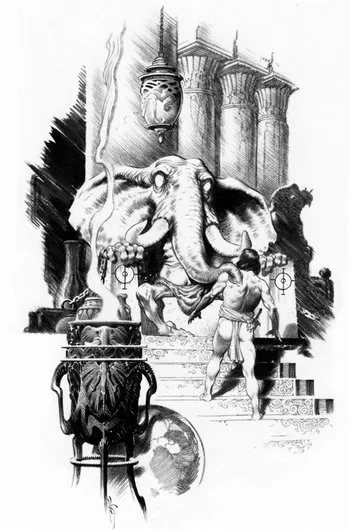
\includegraphics[width=0.5\textwidth]{img/Intro}
\end{figure}
\column[t]{0.5\textwidth}
     \begin{itemize}
         \item Una historia corta de Robert E. Howard
         \item Una de sus mejores historias
         \item Espada y hechicería pura
         \begin{itemize}
          \item Ilustración de Mark Schultz
         \end{itemize}
     \end{itemize}
\end{columns}
\end{frame}

\begin{frame}{Publicación}
\begin{columns}
\column[t]{0.4\textwidth}
    \begin{figure}[htb]
    \centering
        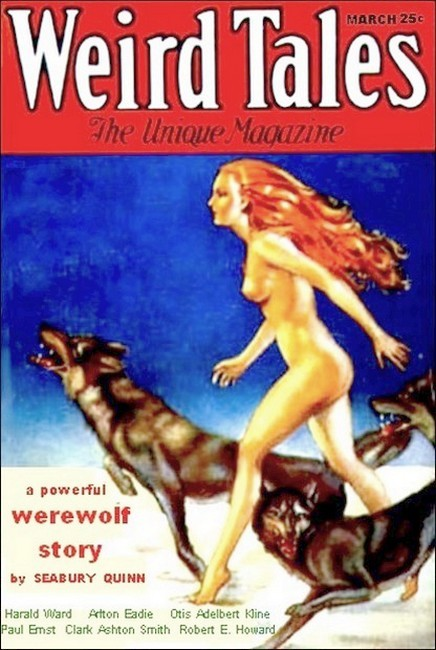
\includegraphics[width=0.5\textwidth]{img/WeirdTales-1933-03}
        \caption{Marzo de 1933}
    \end{figure}
\column[t]{0.6\textwidth}
    \begin{itemize}
         \item Publicada por primera vez en Weird Tales
         \item Alrededor de unas 20 páginas
         \begin{itemize}
            \item 9800 palabras en Ingles
            \item 10600 palabras en Español
            \item Lectura en 40-50 minutos
         \end{itemize}
         \item Una historia de su personaje mas famoso: Conan el bárbaro
         \item Muchas veces publicada en Español y en el idioma original
    \end{itemize}
\end{columns}
\end{frame}

\begin{frame}{Publicación}
	\begin{columns}
		\column[t]{0.4\textwidth}
		\begin{figure}[htb]
			\centering
			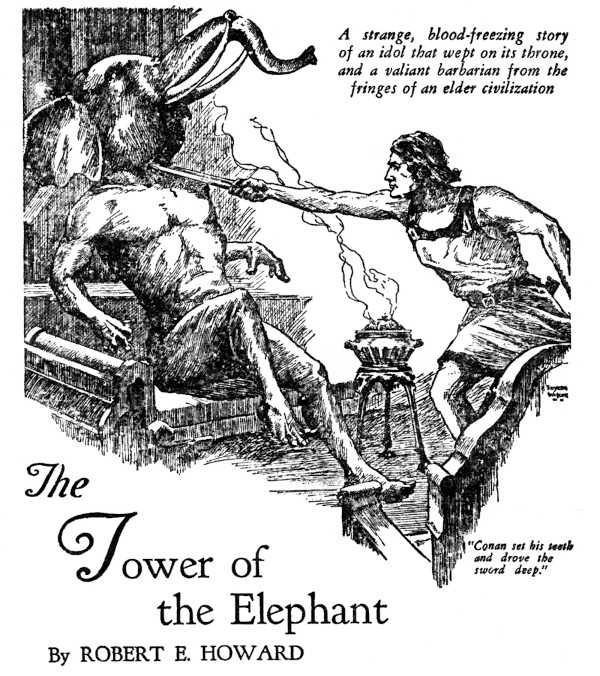
\includegraphics[width=0.75\textwidth]{img/JayemWilcoxTowerOfTheElephant}
			\caption{Jayem Wilcox}
		\end{figure}
		\column[t]{0.6\textwidth}
		\begin{itemize}
			\item Esta ilustración acompaña a la primera edición de la historia
			\item La primera ilustración del relato
		\end{itemize}
	\end{columns}
\end{frame}

\begin{frame}{Orden de publicación del ciclo de Conan}
\begin{figure}[htb]
  \centering
  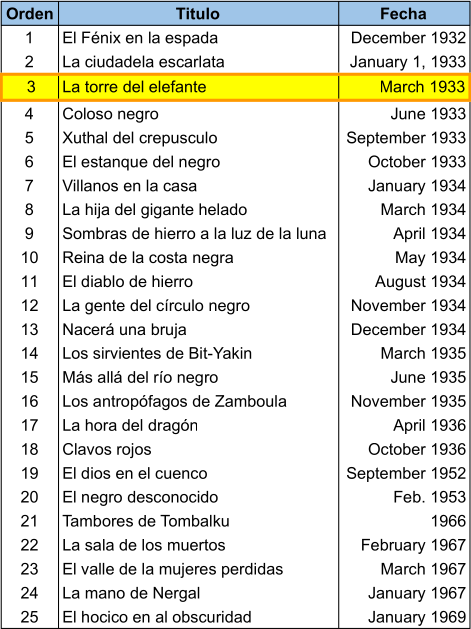
\includegraphics[width=0.32\textwidth]{img/OrdenPublicacion}
\end{figure}
\end{frame}

\begin{frame}{Cronología ficticia del personaje}
\begin{figure}[htb]
  \centering
  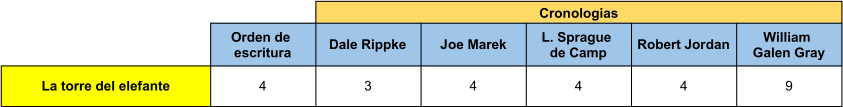
\includegraphics[width=0.85\textwidth]{img/Cronollogias}
\end{figure}
\end{frame}

\begin{frame}{Espacio en la edad Hiboria}
\begin{figure}[htp]
 \centering
 \begin{subfigure}[b]{0.48\textwidth}
   \includegraphics[width=\textwidth]{img/mapas/todo}
   %\caption{Barry Windsor Smith}
 \end{subfigure}
~
 \begin{subfigure}[b]{0.48\textwidth}
   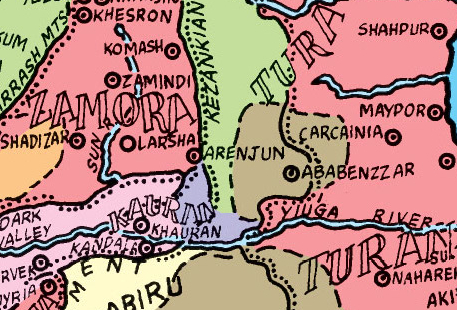
\includegraphics[width=\textwidth]{img/mapas/inset}
   %\caption{Silvio \say{Sal} Buscema}
 \end{subfigure}
 \caption{La ciudad de Arenjun en la provincia de Zamora. La \say{ciudad de los ladrones}}
 \end{figure}
\end{frame}

\section{Adaptaciones}

\begin{frame}{Conan the barbarian}
\begin{columns}
\column[t]{0.4\textwidth}
    \begin{figure}[htb]
    \centering
        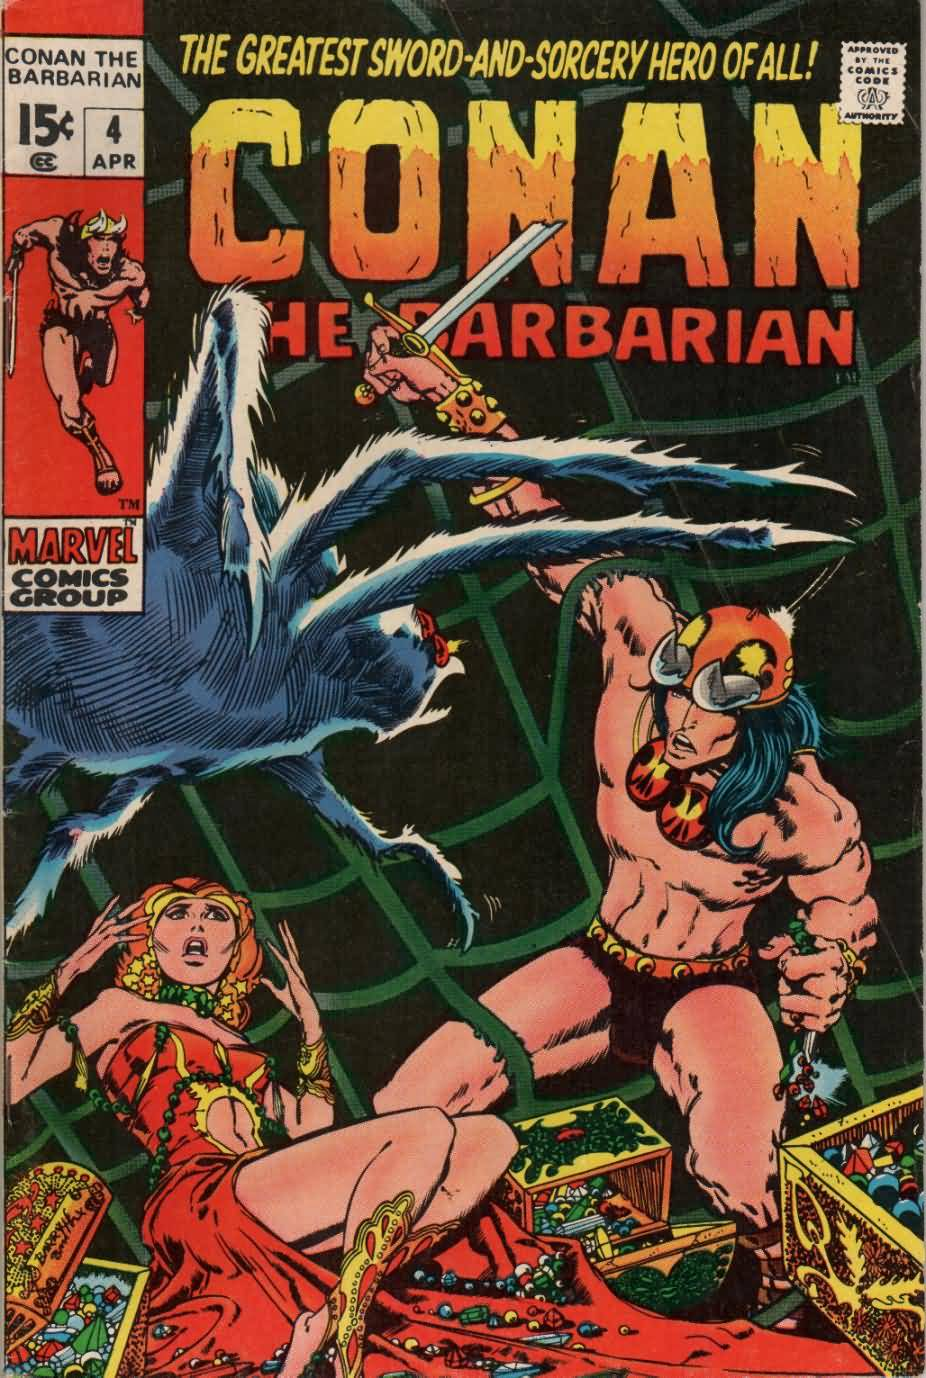
\includegraphics[width=0.55\textwidth]{img/TheBarbarian004Portada}
        \caption{26 de Enero de 1971}
    \end{figure}
\column[t]{0.6\textwidth}
    \begin{itemize}
         \item Número 4 en la serie
         \item 21 páginas
         \item Créditos:
         \begin{description}
            \item[Dibujante:] Barry Windsor Smith
            \item[Entintador:] Silvio \say{Sal} Buscema
            \item[Escritor:] Roy Thomas
            \item[Letrista:] Sam Rosen
            \item[Editor:] Stand Lee
         \end{description}
    \end{itemize}
\end{columns}
\end{frame}

% \begin{frame}{}
% \begin{figure}[htp]
%  \centering
%  \begin{subfigure}[b]{0.16\textwidth}
%    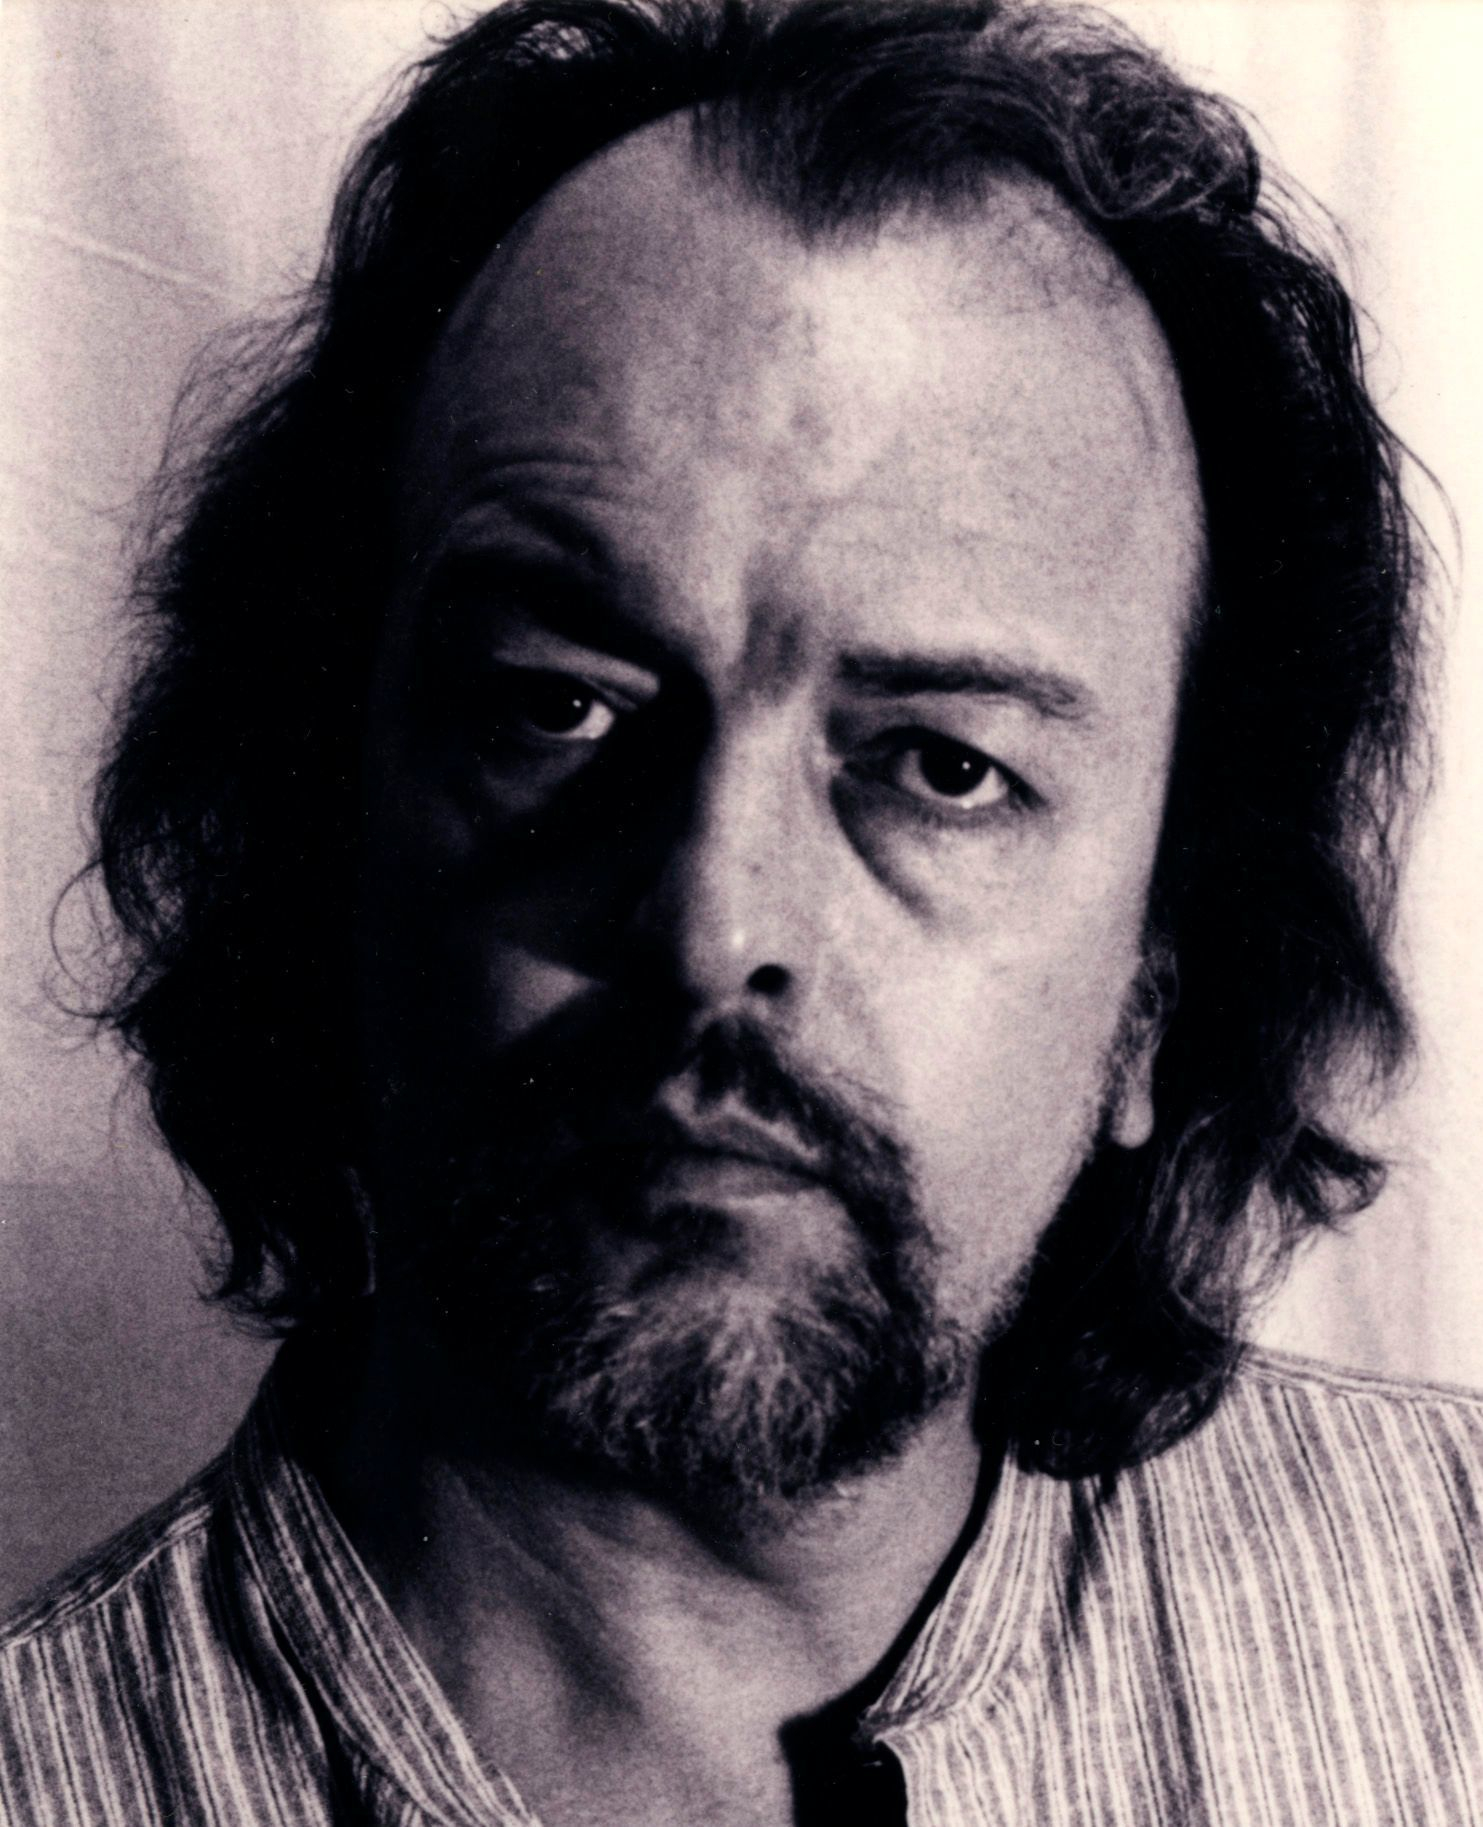
\includegraphics[width=\textwidth]{img/artistas/BarryWindsorSmith}
%    \caption{Barry Windsor Smith}
%  \end{subfigure}
% ~
%  \begin{subfigure}[b]{0.16\textwidth}
%    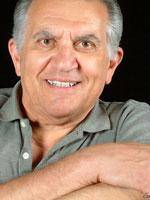
\includegraphics[width=\textwidth]{img/artistas/SalBuscema}
%    \caption{Silvio \say{Sal} Buscema}
%  \end{subfigure}
%  ~
%  \begin{subfigure}[b]{0.16\textwidth}
%    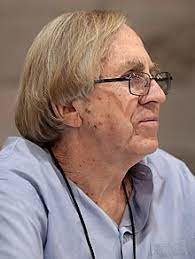
\includegraphics[width=\textwidth]{img/artistas/RoyThomas}
%    \caption{Roy Thomas}
%  \end{subfigure}
% ~
%  \begin{subfigure}[b]{0.16\textwidth}
%    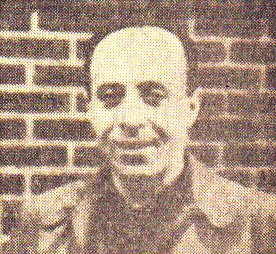
\includegraphics[width=\textwidth]{img/artistas/SamRosen1964}
%    \caption{Sam Rosen}
%  \end{subfigure}
% ~
%  \begin{subfigure}[b]{0.16\textwidth}
%    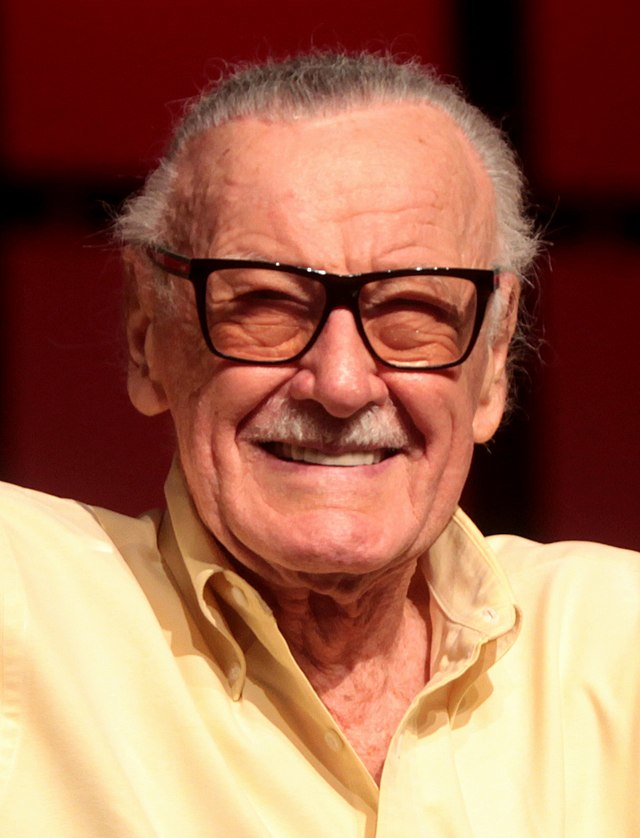
\includegraphics[width=\textwidth]{img/artistas/StanLee}
%    \caption{Stand Lee}
%  \end{subfigure}
% \end{figure}
% \end{frame}


\begin{frame}{The savage sword of Conan}
\begin{columns}
\column[t]{0.4\textwidth}
    \begin{figure}[htb]
    \centering
        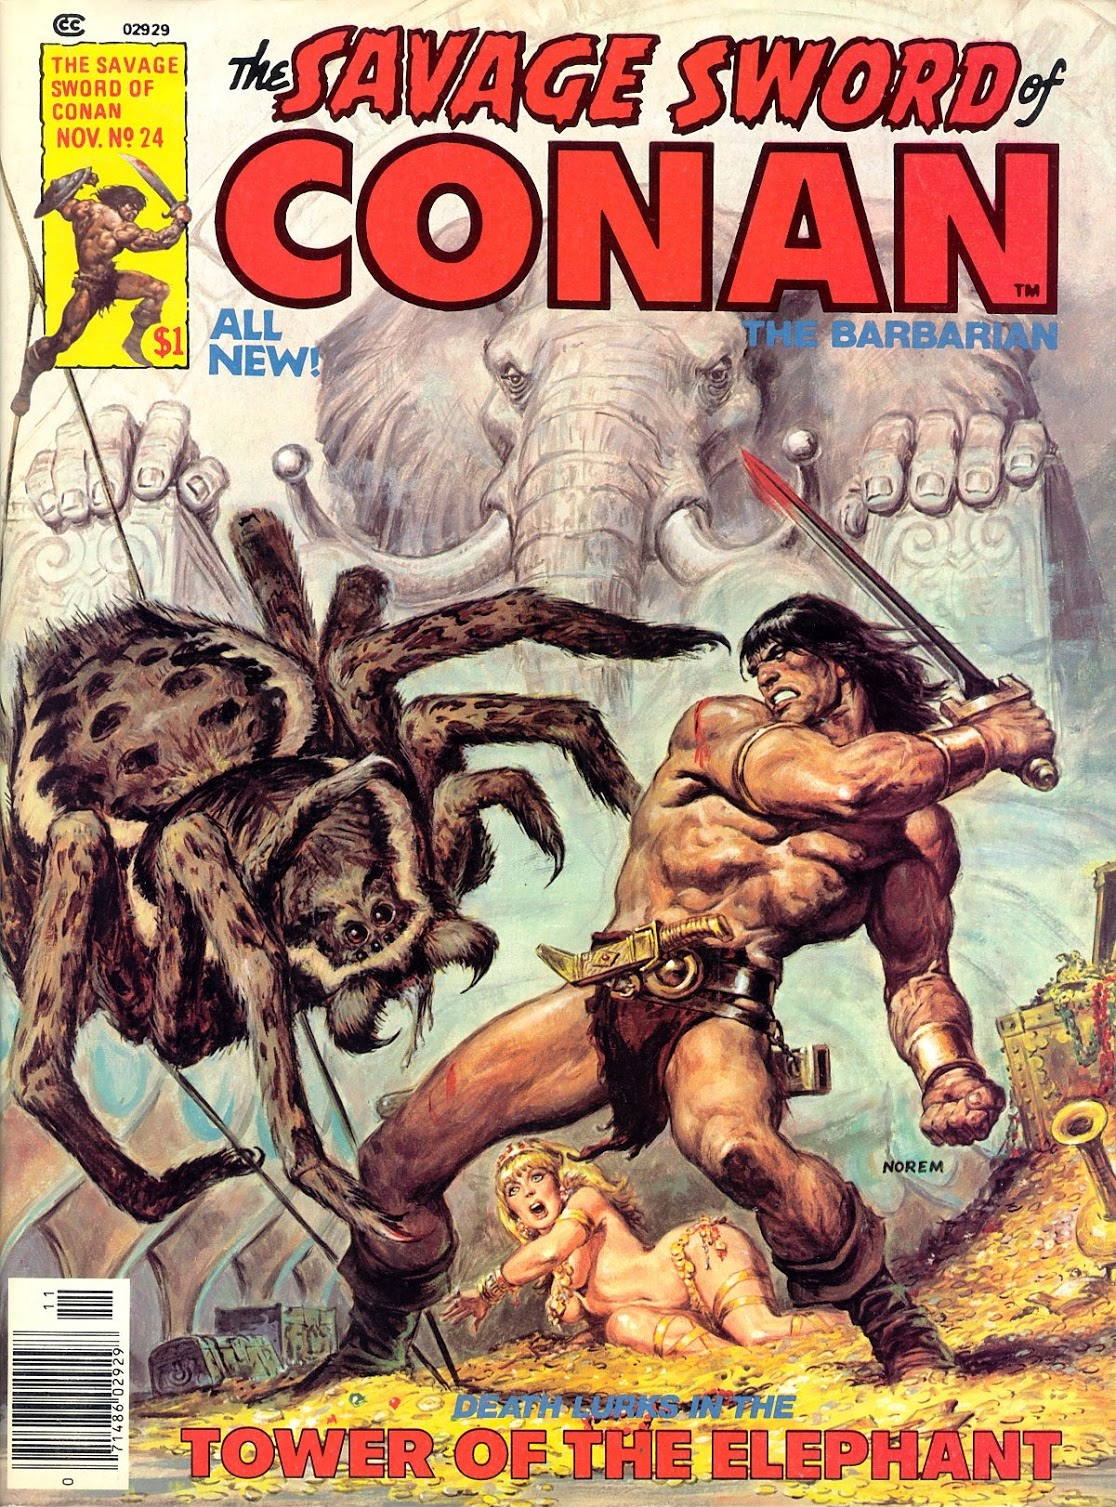
\includegraphics[width=0.6\textwidth]{img/TSSC24Portada}
        \caption{6 de Septiembre de 1977}
    \end{figure}
\column[t]{0.6\textwidth}
    \begin{itemize}
         \item Número 24 en la serie
         \item 65 páginas del ejemplar
         \item 40 de la historia
         \item Créditos:
         \begin{description}
            \item[Artista:] John Buscema
            \item[Artista:] Alfredo Alcalá
            \item[Escritor:] Roy Thomas
            \item[Portada:] Earl Norem
         \end{description}
    \end{itemize}
\end{columns}
\end{frame}

% \begin{frame}{}
% \begin{figure}[htp]
%  \centering
%  \begin{subfigure}[b]{0.16\textwidth}
%    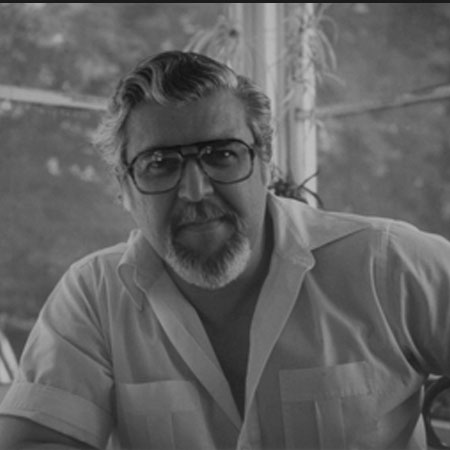
\includegraphics[width=\textwidth]{img/artistas/JohnBuscema}
%    \caption{John Buscema}
%  \end{subfigure}
% ~
%  \begin{subfigure}[b]{0.16\textwidth}
%    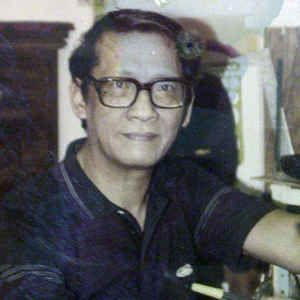
\includegraphics[width=\textwidth]{img/artistas/AlfredoAlcala}
%    \caption{Alfredo Alcalá}
%  \end{subfigure}
%  ~
%  \begin{subfigure}[b]{0.16\textwidth}
%    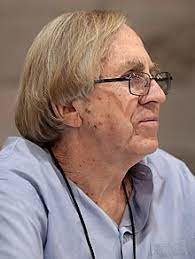
\includegraphics[width=\textwidth]{img/artistas/RoyThomas}
%    \caption{Roy Thomas}
%  \end{subfigure}
% ~
%  \begin{subfigure}[b]{0.16\textwidth}
%    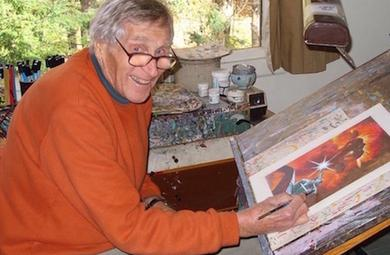
\includegraphics[width=\textwidth]{img/artistas/EarlNorem}
%    \caption{Earl Norem}
%  \end{subfigure}
% \end{figure}
% \end{frame}

\begin{frame}{Conan}
\begin{columns}
\column[t]{0.6\textwidth}
\begin{figure}[htp]
 \centering
 \begin{subfigure}[b]{0.3\textwidth}
   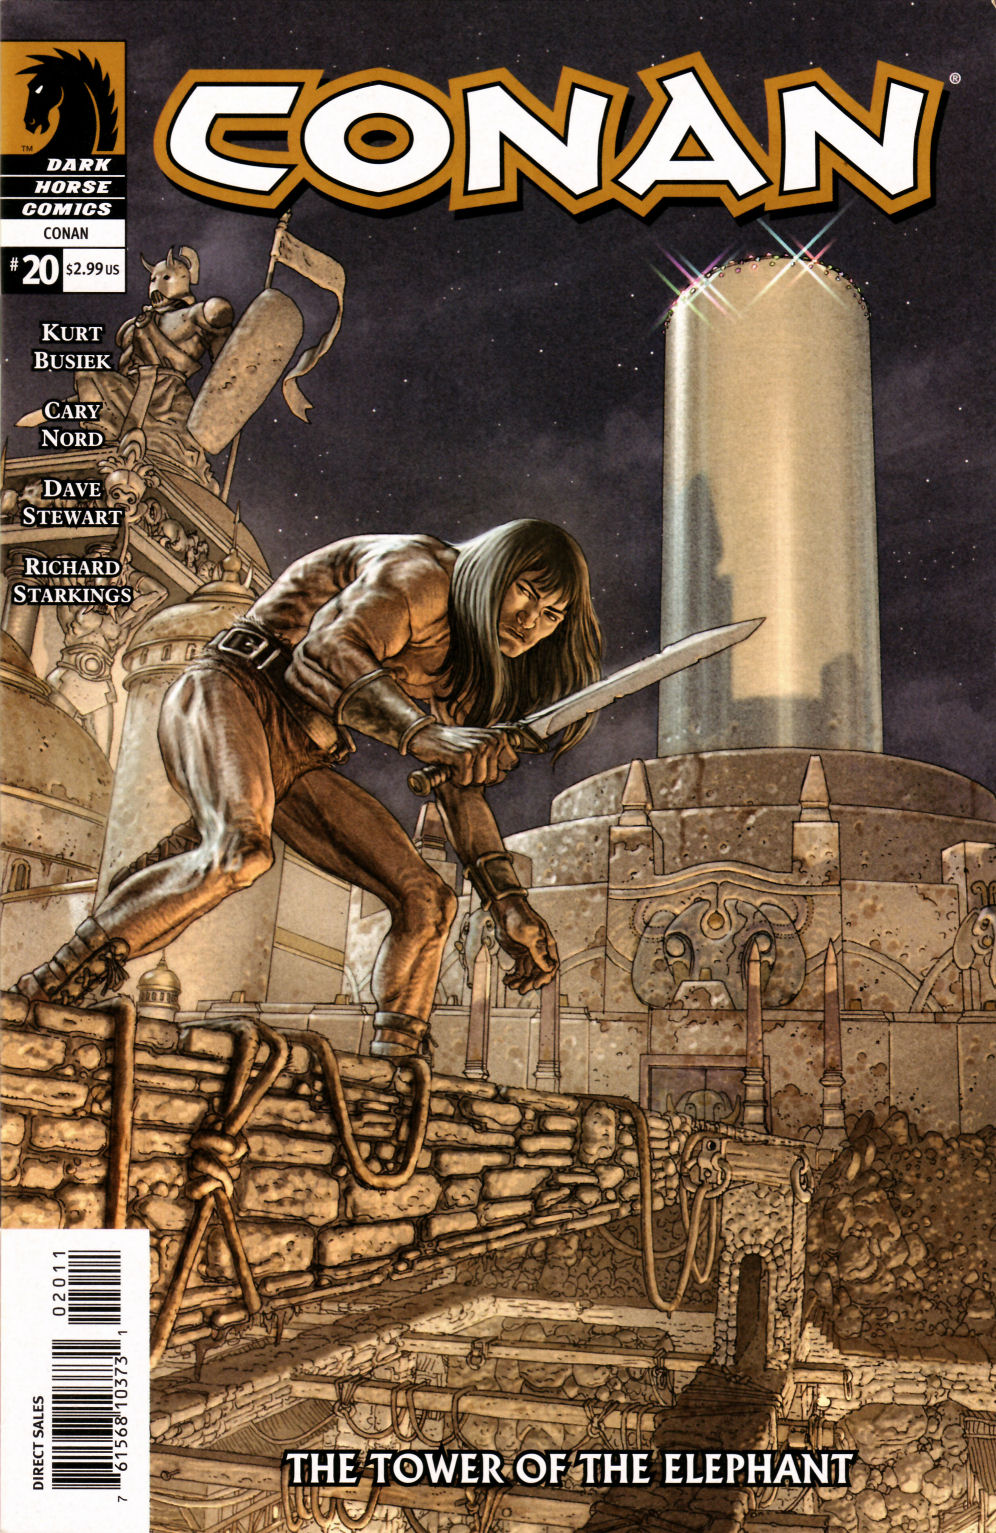
\includegraphics[width=\textwidth]{img/DarkHorse20Portada}
   \caption{Septiembre}
 \end{subfigure}
~
 \begin{subfigure}[b]{0.3\textwidth}
   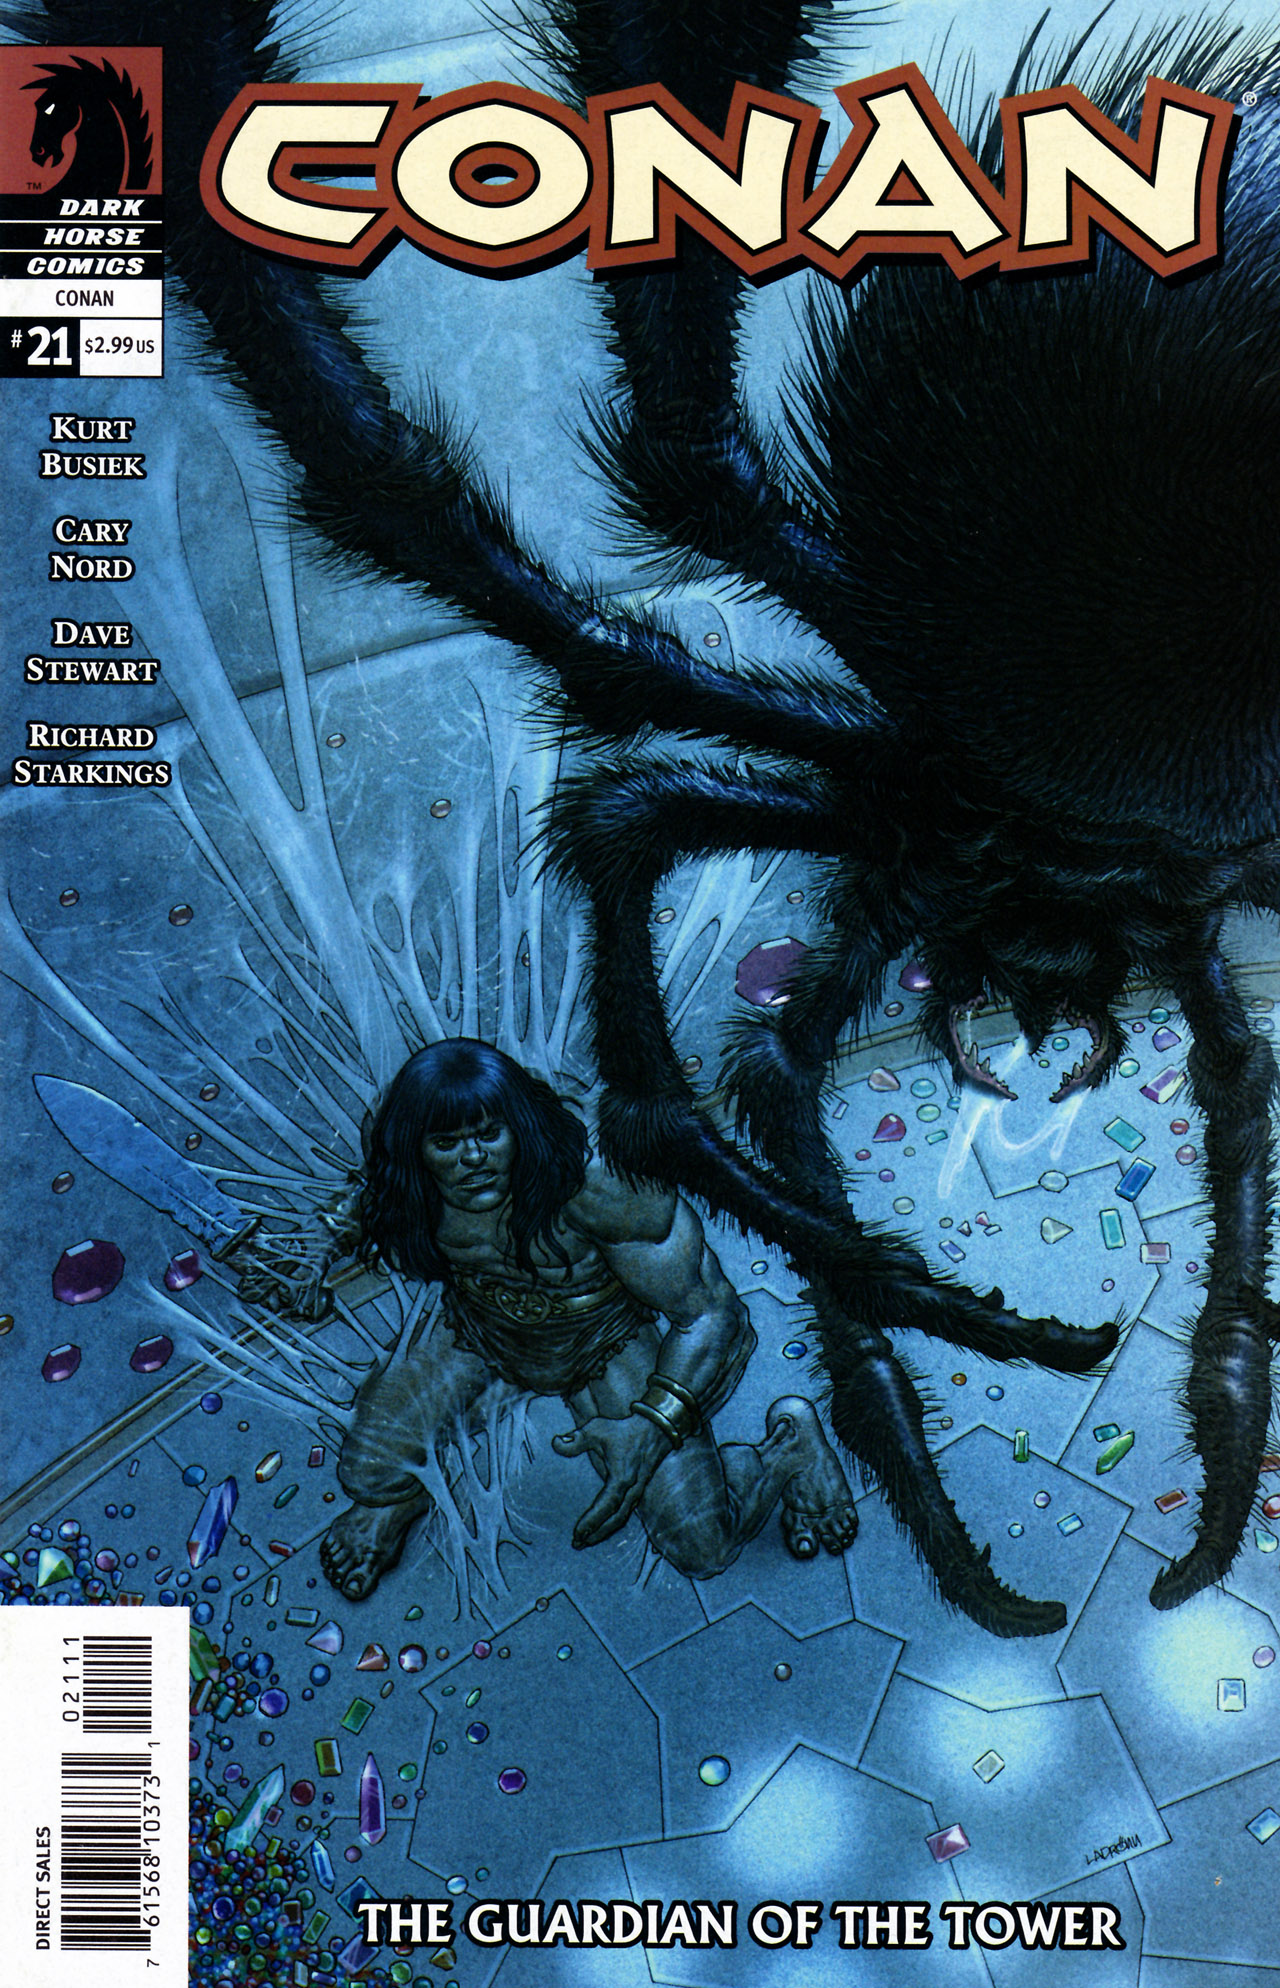
\includegraphics[width=\textwidth]{img/DarkHorse21Portada}
   \caption{Octubre}
 \end{subfigure}
 ~
 \begin{subfigure}[b]{0.3\textwidth}
   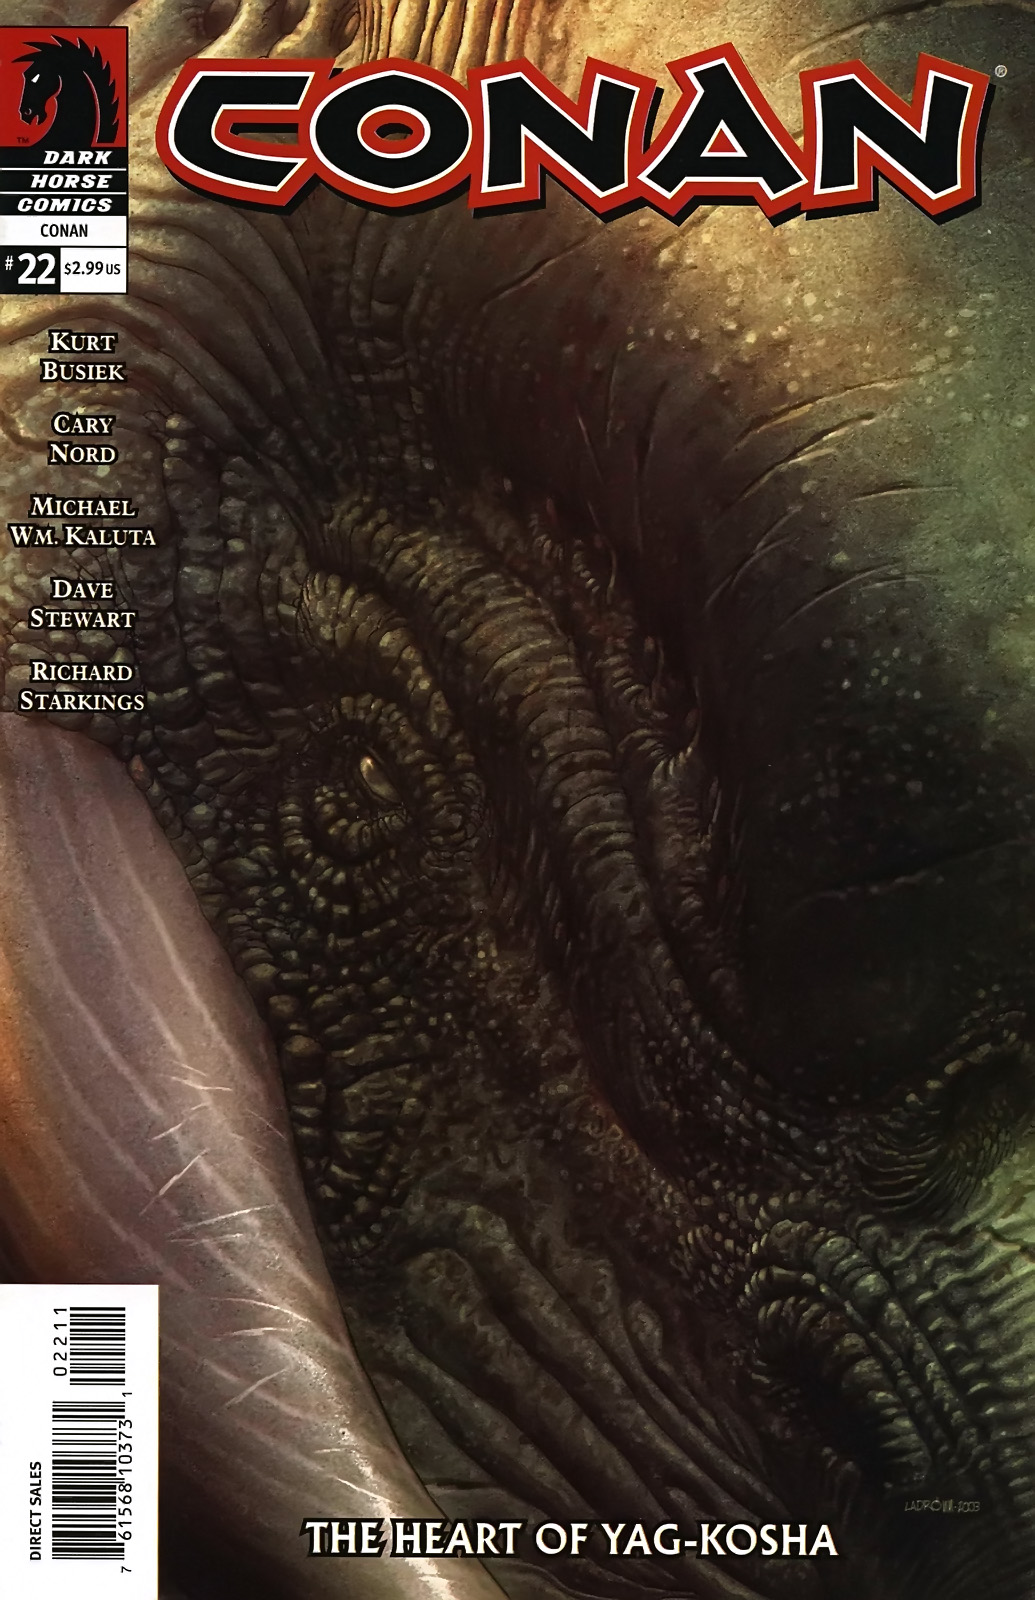
\includegraphics[width=\textwidth]{img/DarkHorse22Portada}
   \caption{Noviembre}
 \end{subfigure}
\end{figure}
\begin{center}
2005
\end{center}
\column[t]{0.4\textwidth}
    \begin{itemize}
         \item \say{Conan de Dark Horse}
         \item Números 20, 21 y 22 en la serie
         \item 23, 25 y 26 pp. en cada ejemplar
         \item 20, 22 y 23 de la historia
         \item Créditos:
         \begin{description}
            \item[Artista:] Cary Nord
            \item[Artista(6pp):] Michael Kaluta
            \item[Escritor:] Kurt Busiek
            \item[Colorista:] Dave Steward
            \item[Portada:] José Ladrönn
            \item[Letrista:] Richard Starkings
         \end{description}
    \end{itemize}
\end{columns}
\end{frame}

\begin{frame}{Acción comics: La torre del elefante}
	\begin{columns}
		\column[t]{0.4\textwidth}
		\begin{figure}[htb]
			\centering
			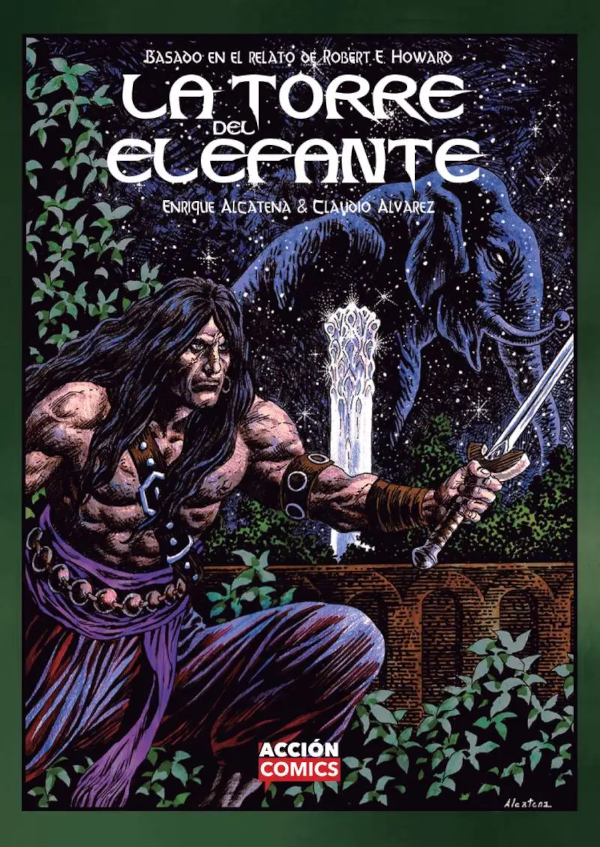
\includegraphics[width=0.6\textwidth]{img/AlcatenaTorre}
			\caption{Marzo 2025}
		\end{figure}
		\column[t]{0.6\textwidth}
		\begin{itemize}
			\item Tomo único
			\item Comic editado en Chile
			\item 76 páginas en Blanco y Negro
			\item Créditos:
			\begin{description}
				\item[Artista:] Enrique Alcatena
				\item[Escritor:] Claudio Álvarez
			\end{description}
		\end{itemize}
	\end{columns}
\end{frame}


\begin{frame}{Conan illustré: La Tour de l’Eléphant}
	\begin{columns}
		\column[t]{0.4\textwidth}
		\begin{figure}[htb]
			\centering
			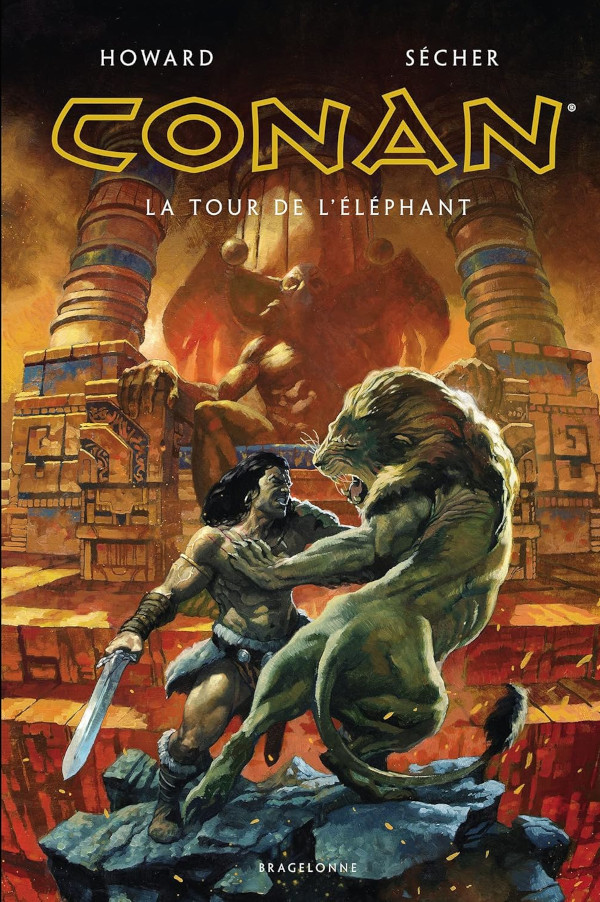
\includegraphics[width=0.6\textwidth]{img/SecherTorre}
			\caption{Octubre 2022}
		\end{figure}
		\column[t]{0.6\textwidth}
		\begin{itemize}
			\item No es una adaptación, es una edición ilustrada.
			\item Edición original en francés
			\item 56 páginas
			\item Créditos:
			\begin{description}
				\item[Artista:] Valentin Sécher
			\end{description}
		\end{itemize}
	\end{columns}
\end{frame}
% \begin{frame}{}
% \begin{figure}[htp]
%  \centering
%  \begin{subfigure}[b]{0.17\textwidth}
%    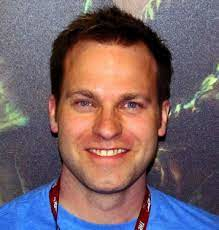
\includegraphics[width=\textwidth]{img/artistas/CaryNord}
%    \caption{Cary Nord}
%  \end{subfigure}
% ~
%  \begin{subfigure}[b]{0.17\textwidth}
%    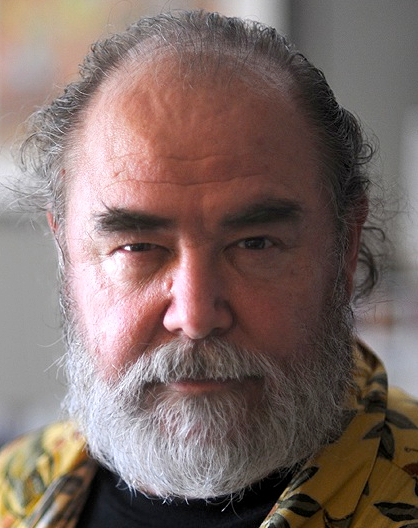
\includegraphics[width=\textwidth]{img/artistas/MichaelKaluta}
%    \caption{Michael Kaluta}
%  \end{subfigure}
% ~
%  \begin{subfigure}[b]{0.17\textwidth}
%    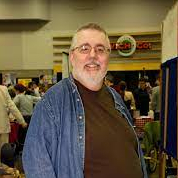
\includegraphics[width=\textwidth]{img/artistas/KurtBusiek}
%    \caption{Kurt Busiek}
%  \end{subfigure}
% \\
%  \begin{subfigure}[b]{0.17\textwidth}
%    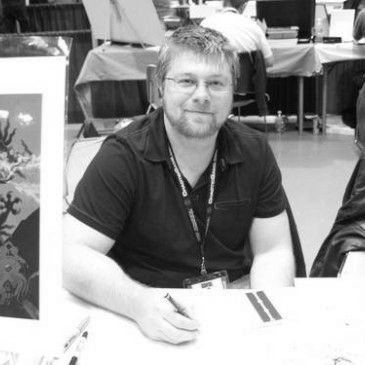
\includegraphics[width=\textwidth]{img/artistas/DaveStewart}
%    \caption{Dave Steward}
%  \end{subfigure}
% ~
%  \begin{subfigure}[b]{0.17\textwidth}
%    
\includegraphics[width=\textwidth]{img/artistas/JoseLadronn}
%    \caption{José Ladrönn}
%  \end{subfigure}
% ~
%  \begin{subfigure}[b]{0.17\textwidth}
%    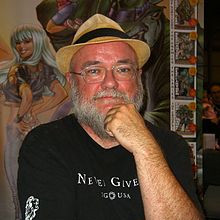
\includegraphics[width=\textwidth]{img/artistas/RichardStarkings}
%    \caption{Richard Starkings}
%  \end{subfigure}
% \end{figure}
% \end{frame}

\section{Resumen}

\begin{frame}{}
\begin{columns}
\column[t]{0.5\textwidth}
    \begin{figure}[htb]
    \centering
        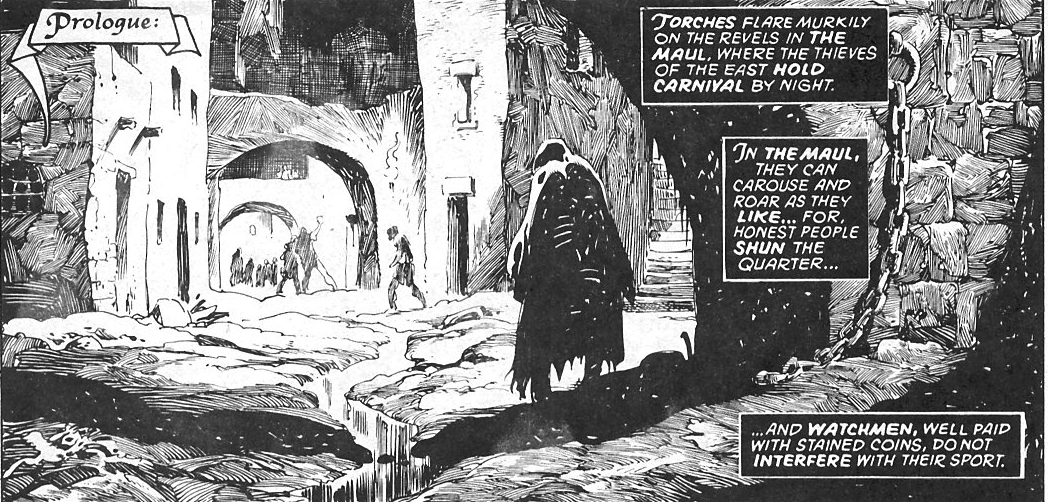
\includegraphics[width=0.9\textwidth]{img/res/01}
        \caption{El Maul}
    \end{figure}
\column[t]{0.5\textwidth}
    \begin{figure}[htb]
    \centering
        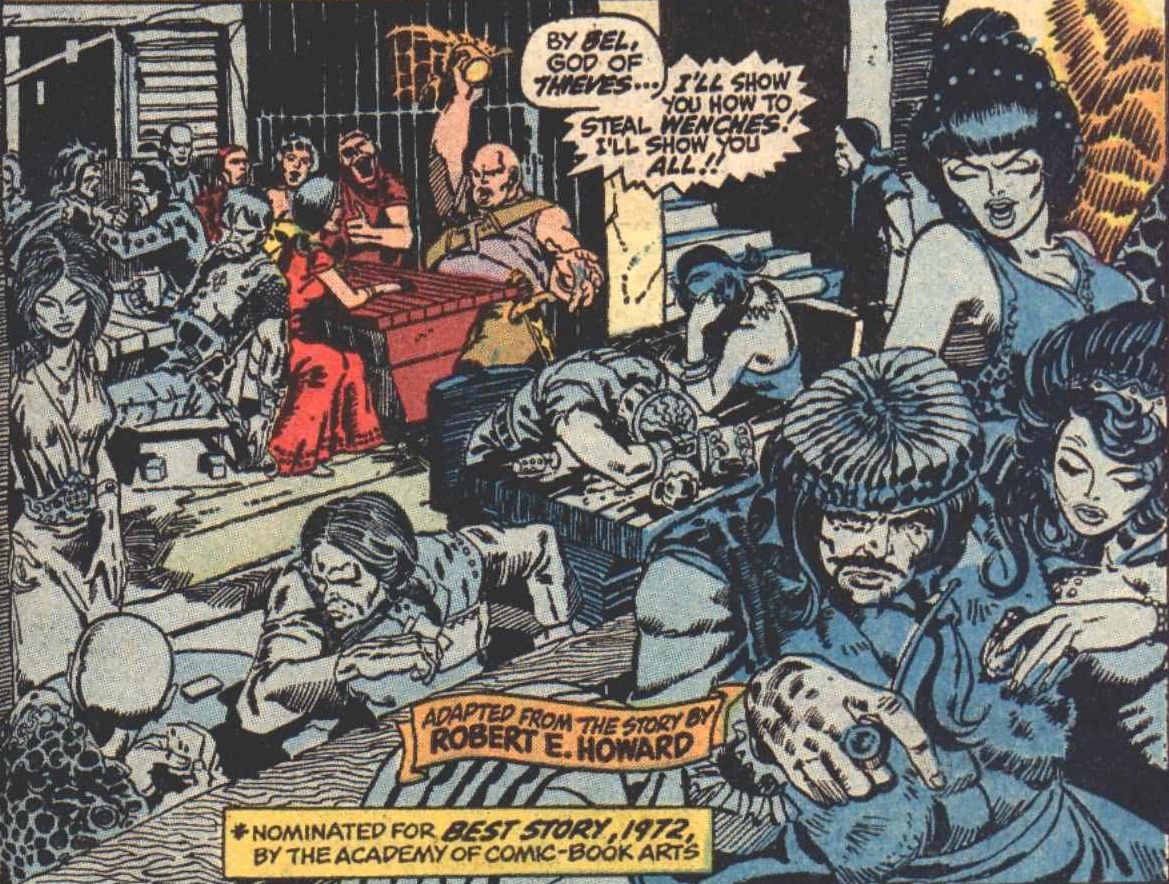
\includegraphics[width=0.9\textwidth]{img/res/02}
        \caption{Una taberna}
    \end{figure}
\end{columns}
\end{frame}

\begin{frame}{}
\begin{columns}
\column[t]{0.5\textwidth}
    \begin{figure}[htb]
    \centering
        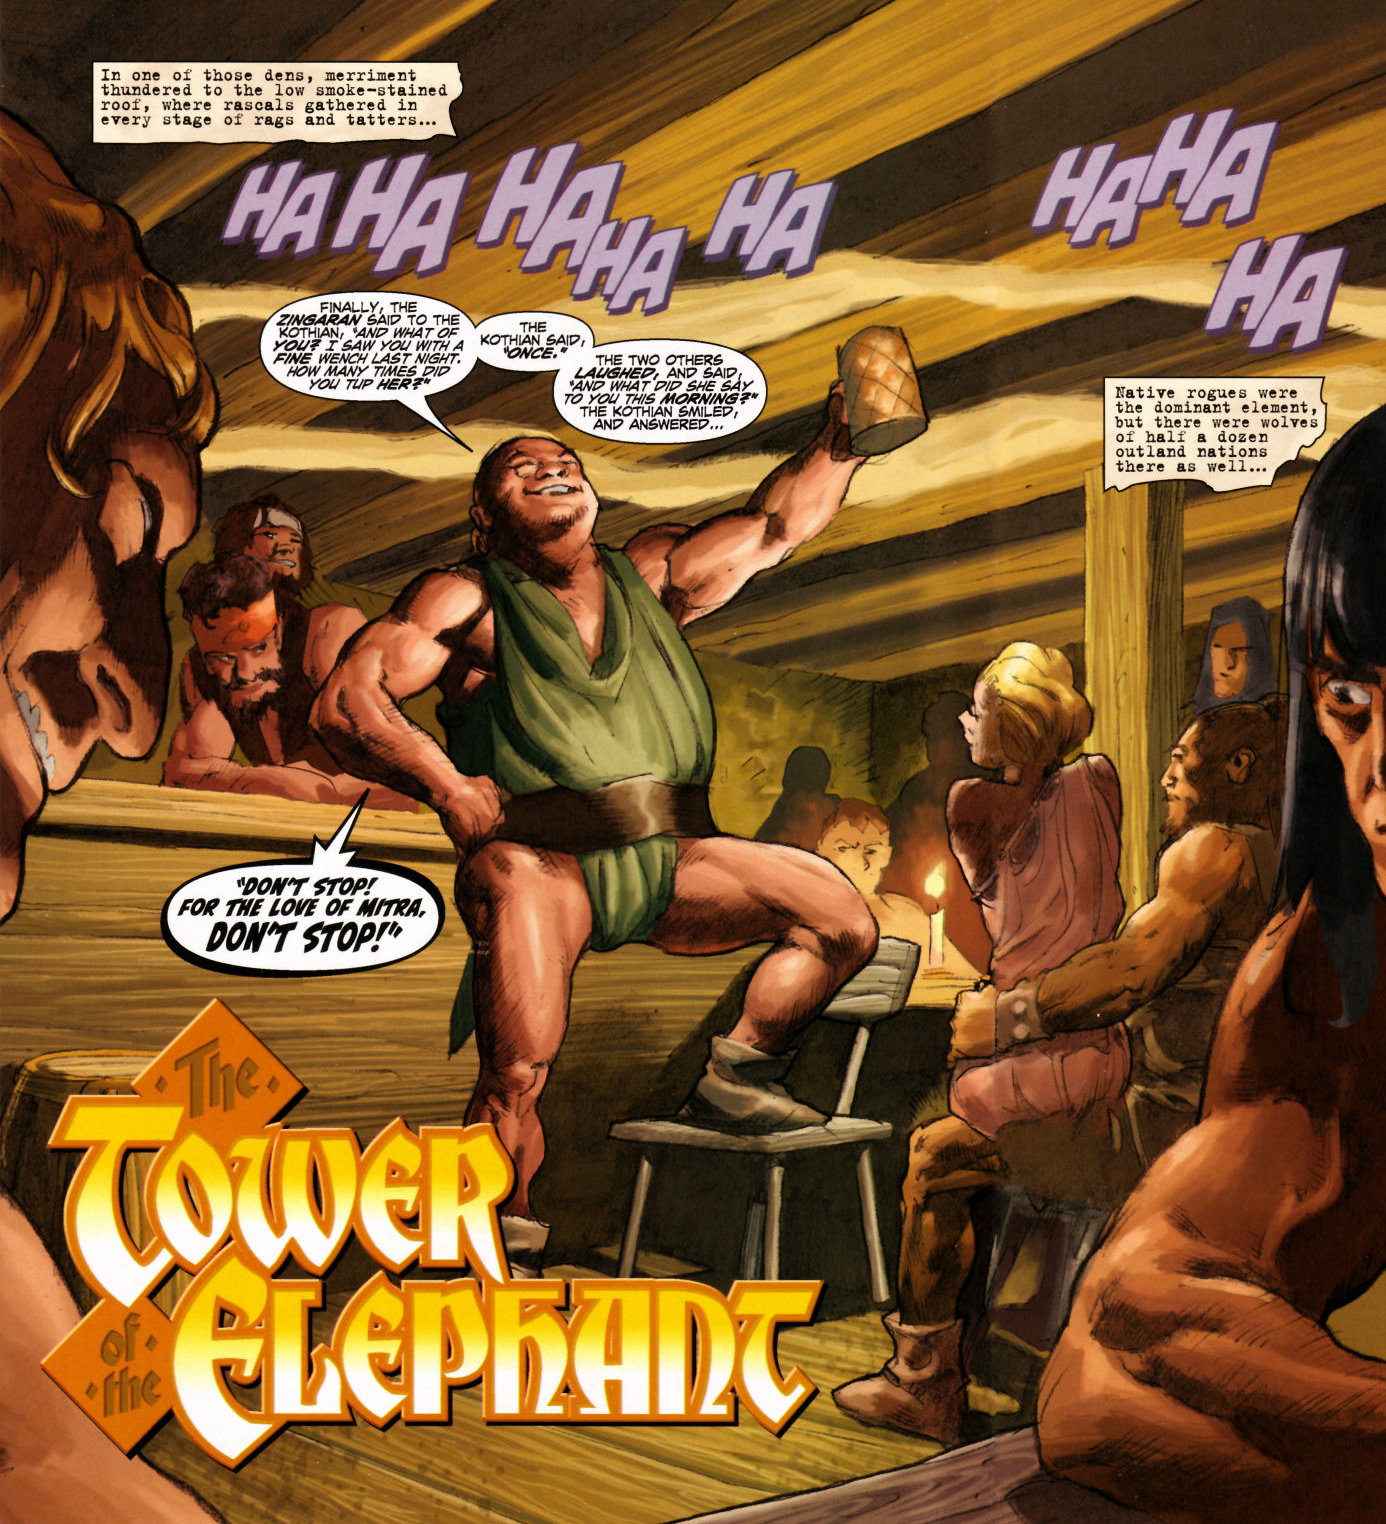
\includegraphics[width=0.65\textwidth]{img/res/03}
        \caption{El Kothio}
    \end{figure}
\column[t]{0.5\textwidth}
    \begin{figure}[htb]
    \centering
        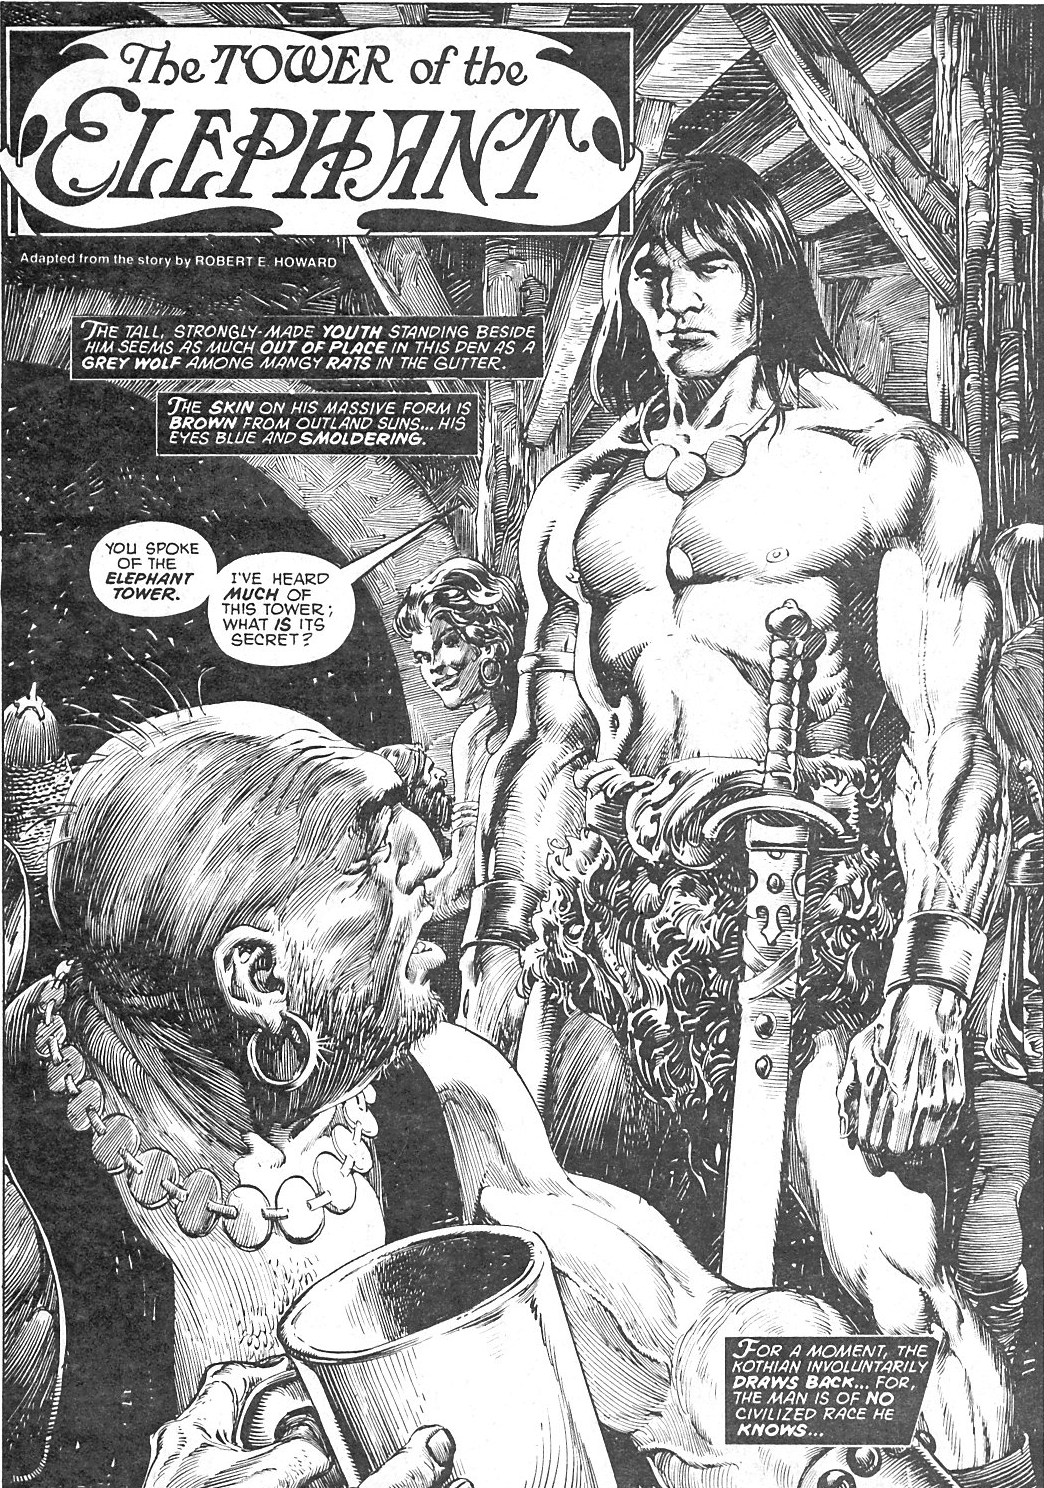
\includegraphics[width=0.55\textwidth]{img/res/04}
        \caption{Conan entra en escena}
    \end{figure}
\end{columns}
\end{frame}

\begin{frame}{}
\begin{columns}
\column[t]{0.5\textwidth}
    \begin{figure}[htb]
    \centering
        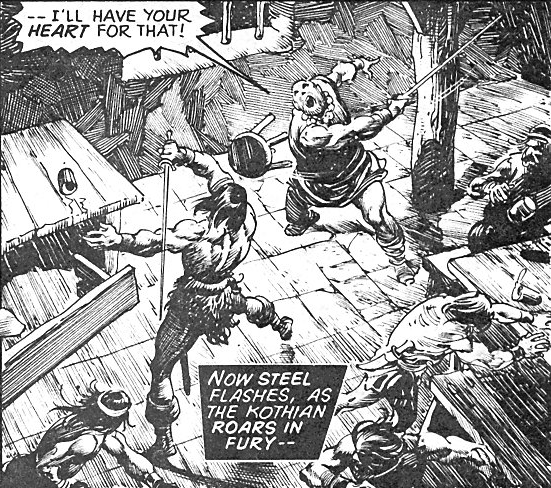
\includegraphics[width=0.7\textwidth]{img/res/05}
        \caption{Una pelea}
    \end{figure}
\column[t]{0.5\textwidth}
    \begin{figure}[htb]
    \centering
        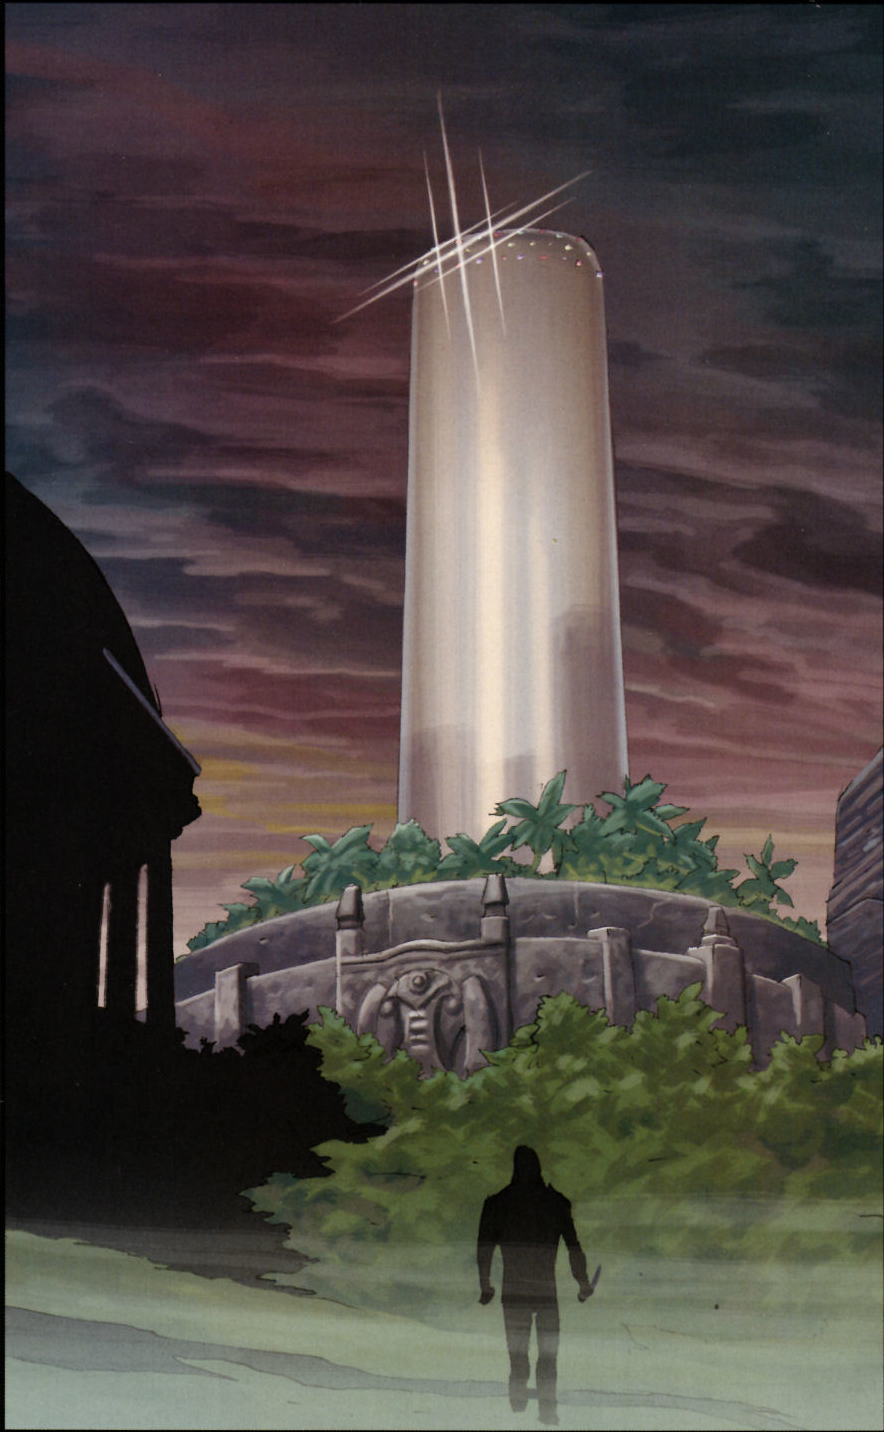
\includegraphics[width=0.4\textwidth]{img/res/06}
        \caption{La torre}
    \end{figure}
\end{columns}
\end{frame}

\begin{frame}{}
\begin{columns}
\column[t]{0.5\textwidth}
    \begin{figure}[htb]
    \centering
        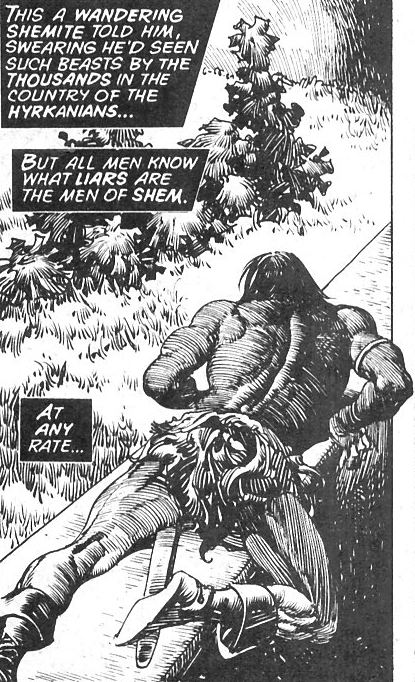
\includegraphics[width=0.5\textwidth]{img/res/07}
        \caption{El muro exterior}
    \end{figure}
\column[t]{0.5\textwidth}
    \begin{figure}[htb]
    \centering
        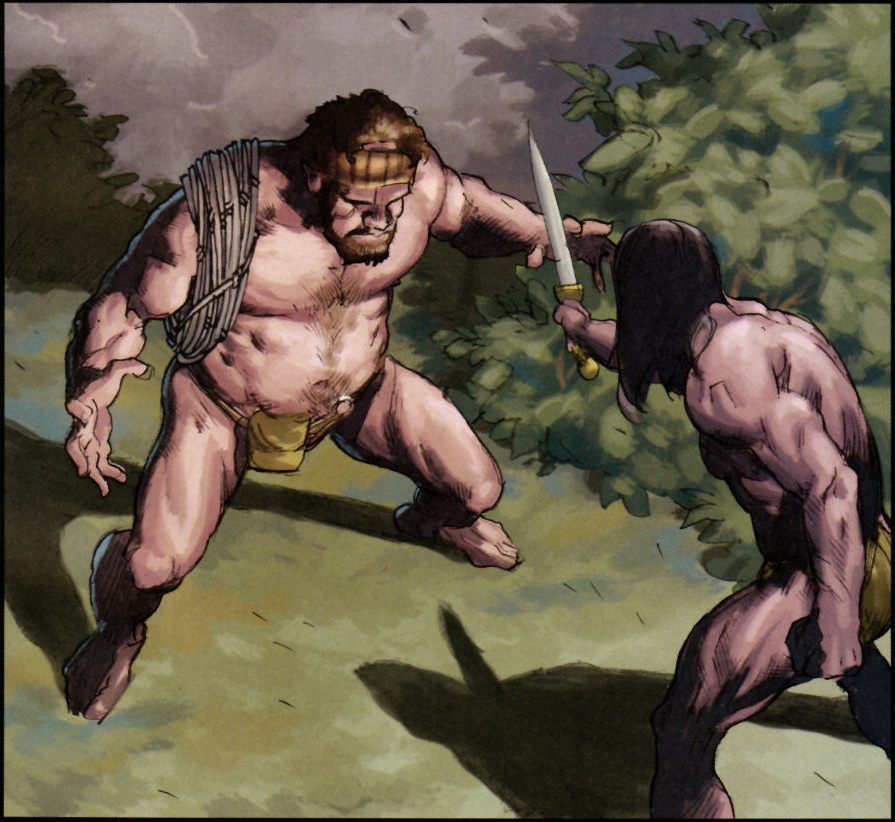
\includegraphics[width=0.7\textwidth]{img/res/08}
        \caption{Tauros de Nemedia}
    \end{figure}
\end{columns}
\end{frame}

\begin{frame}{}
\begin{columns}
\column[t]{0.7\textwidth}
    \begin{figure}[htb]
    \centering
        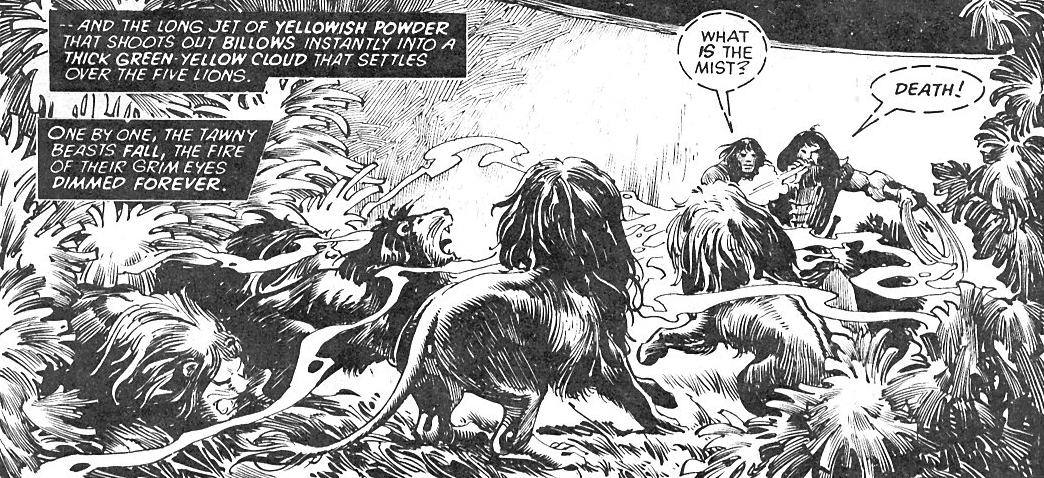
\includegraphics[width=0.85\textwidth]{img/res/09}
        \caption{Los guardianes del jardín}
    \end{figure}
\column[t]{0.3\textwidth}
    \begin{figure}[htb]
    \centering
        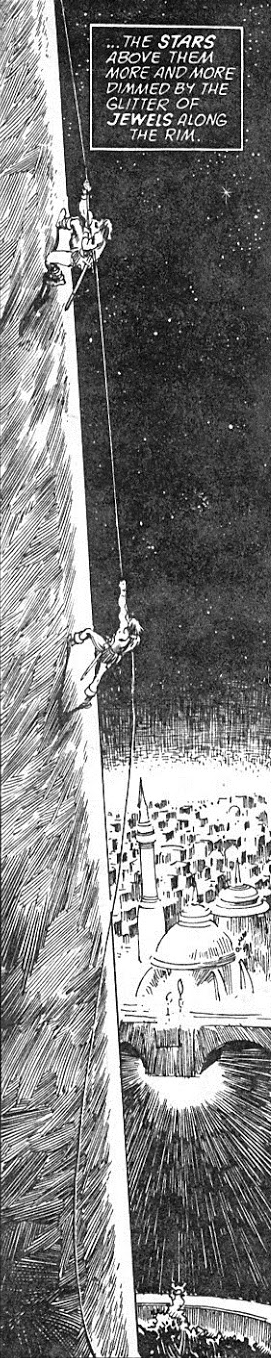
\includegraphics[width=0.28\textwidth]{img/res/10}
        \caption{Escalada}
    \end{figure}
\end{columns}
\end{frame}

\begin{frame}{}
\begin{columns}
\column[t]{0.5\textwidth}
    \begin{figure}[htb]
    \centering
        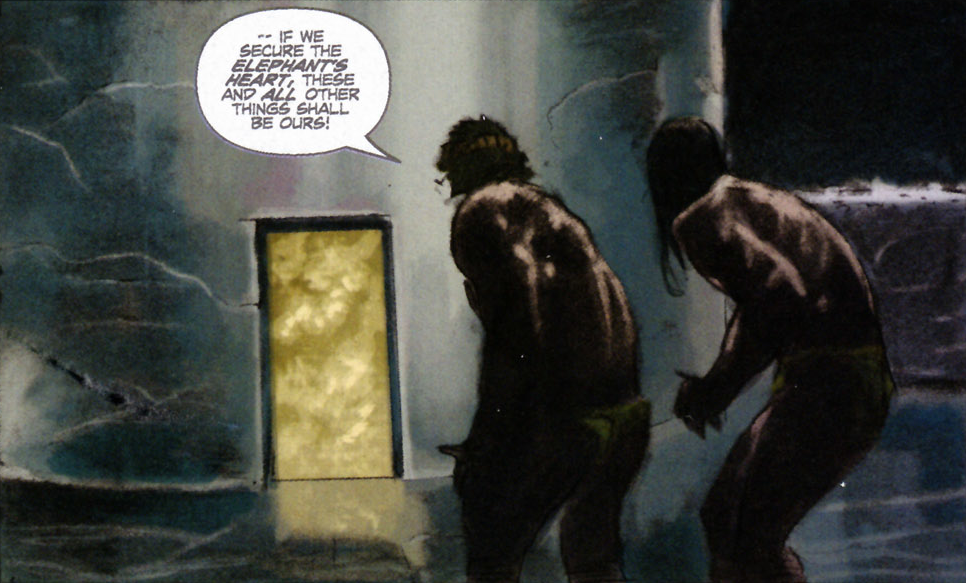
\includegraphics[width=0.8\textwidth]{img/res/11}
        \caption{Una puerta sin cerrojo}
    \end{figure}
\column[t]{0.5\textwidth}
    \begin{figure}[htb]
    \centering
        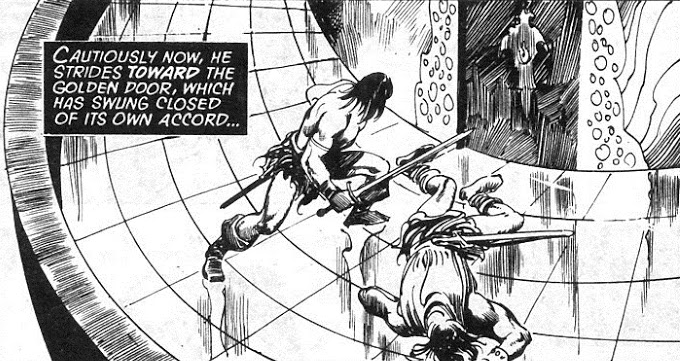
\includegraphics[width=0.9\textwidth]{img/res/12}
        \caption{El fin de Tauros}
    \end{figure}
\end{columns}
\end{frame}

\begin{frame}{}
\begin{columns}
\column[t]{0.4\textwidth}
    \begin{figure}[htb]
    \centering
        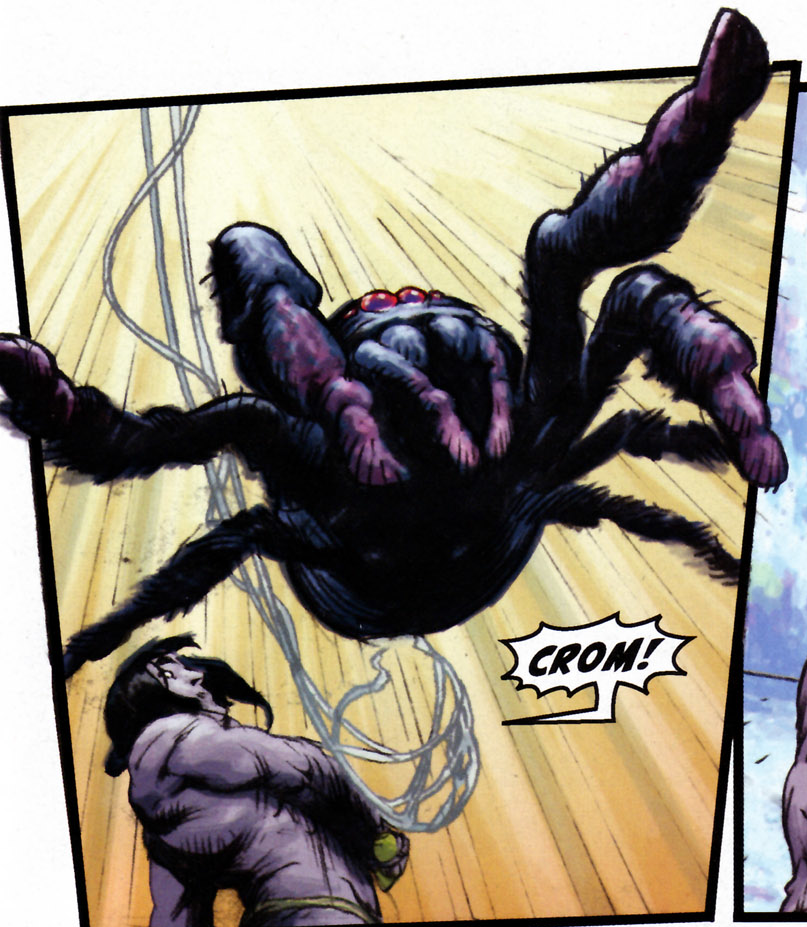
\includegraphics[width=0.7\textwidth]{img/res/13}
        \caption{El guardian de la torre}
    \end{figure}
\column[t]{0.6\textwidth}
    \begin{figure}[htb]
    \centering
        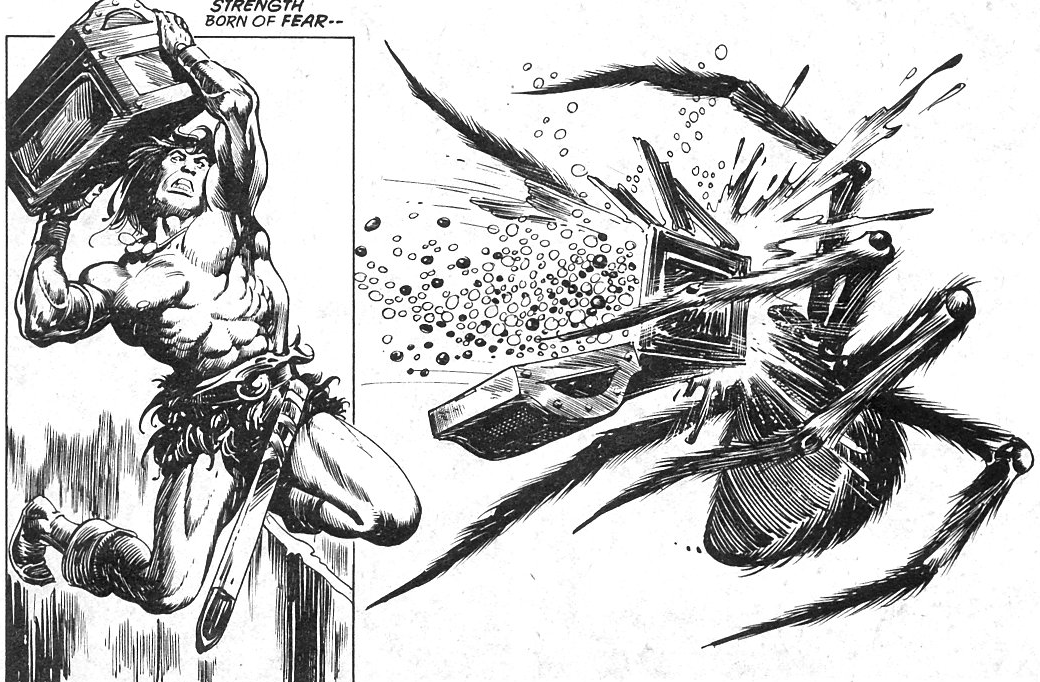
\includegraphics[width=0.85\textwidth]{img/res/14}
        \caption{Una muerte fortuita}
    \end{figure}
\end{columns}
\end{frame}

\begin{frame}{}
\begin{columns}
\column[t]{0.6\textwidth}
    \begin{figure}[htb]
    \centering
        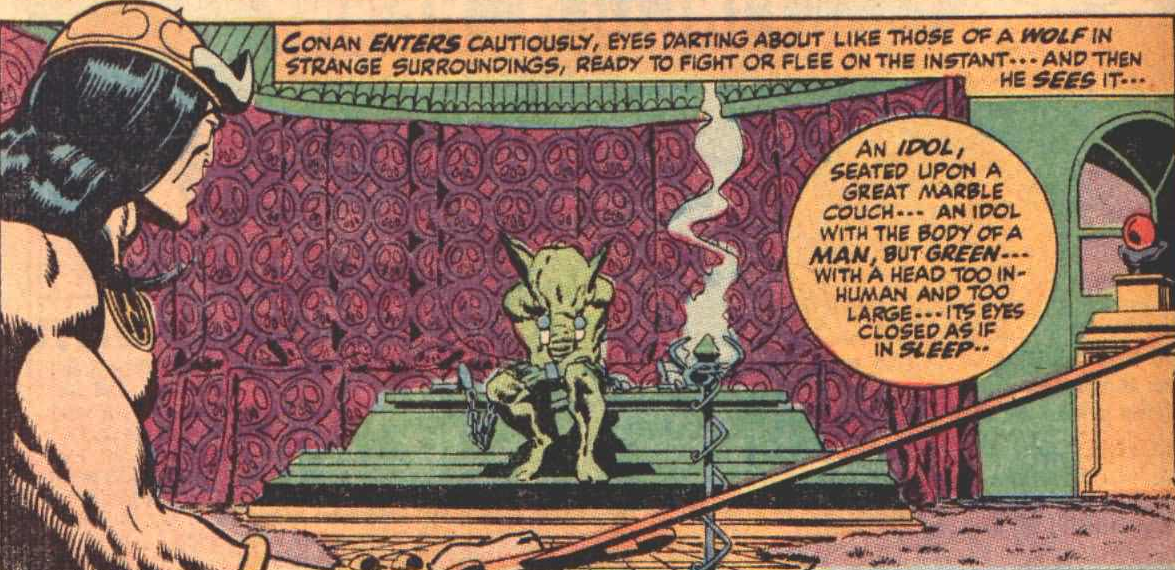
\includegraphics[width=0.85\textwidth]{img/res/15}
        \caption{El cautivo}
    \end{figure}
\column[t]{0.4\textwidth}
    \begin{figure}[htb]
    \centering
        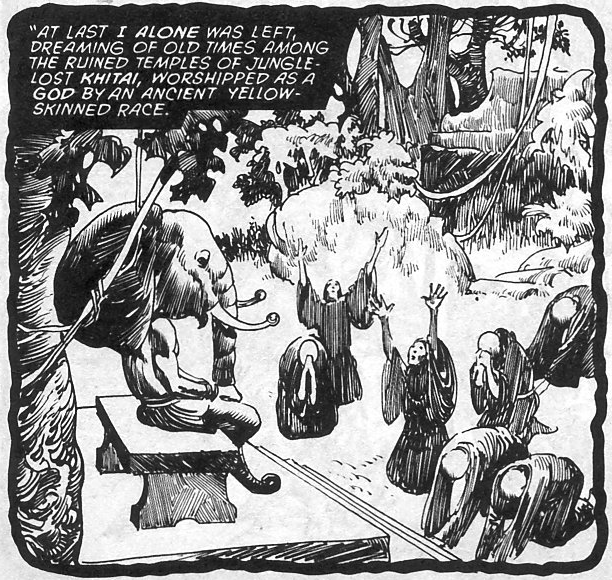
\includegraphics[width=0.85\textwidth]{img/res/16}
        \caption{Era venerado como un díos}
    \end{figure}
\end{columns}
\end{frame}

\begin{frame}{}
\begin{columns}
\column[t]{0.4\textwidth}
    \begin{figure}[htb]
    \centering
        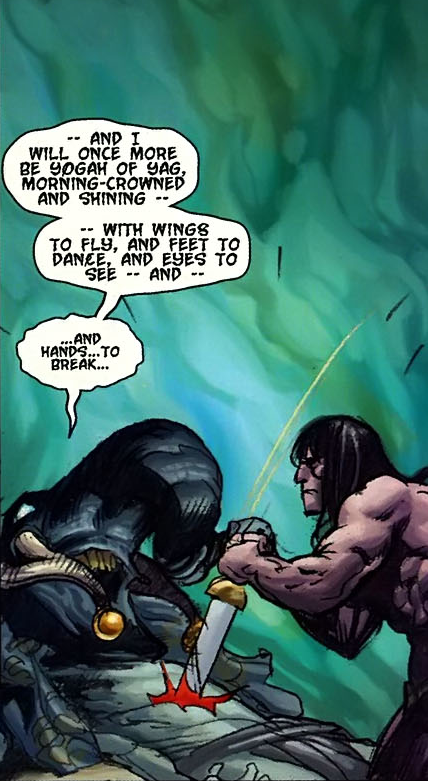
\includegraphics[width=0.55\textwidth]{img/res/17}
        \caption{Una muerte piadosa}
    \end{figure}
\column[t]{0.6\textwidth}
    \begin{figure}[htb]
    \centering
        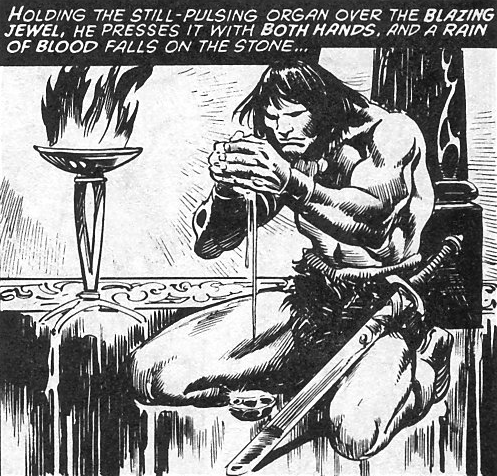
\includegraphics[width=0.7\textwidth]{img/res/18}
        \caption{El corazón y la sangre}
    \end{figure}
\end{columns}
\end{frame}

\begin{frame}{}
\begin{columns}
\column[t]{0.3\textwidth}
    \begin{figure}[htb]
    \centering
        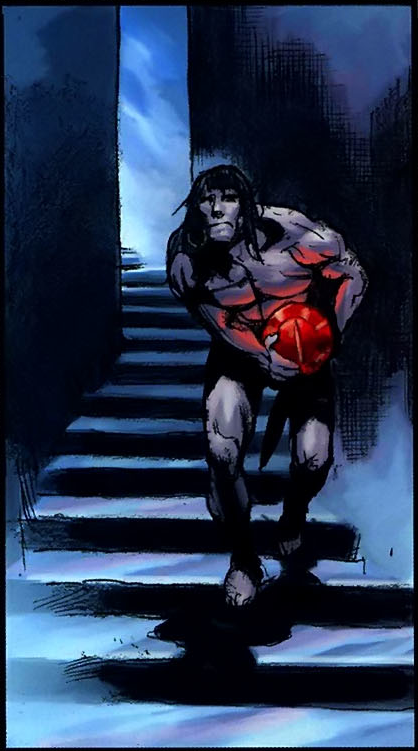
\includegraphics[width=0.7\textwidth]{img/res/19}
        \caption{Una promesa}
    \end{figure}
\column[t]{0.7\textwidth}
    \begin{figure}[htb]
    \centering
        \includegraphics[width=0.8\textwidth]{img/res/20}
        \caption{La venganza de Yag-Kosha}
    \end{figure}
\end{columns}
\end{frame}

\begin{frame}{}
\begin{columns}
\column[t]{0.5\textwidth}
    \begin{figure}[htb]
    \centering
        \includegraphics[width=0.8\textwidth]{img/res/21}
        \caption{El fin de Yaga}
    \end{figure}
\column[t]{0.5\textwidth}
    \begin{figure}[htb]
    \centering
        \includegraphics[width=0.5\textwidth]{img/res/22}
        \caption{La torre se derrumba}
    \end{figure}
\end{columns}
\end{frame}

\section{Personajes}
\begin{frame}{Conan}
\begin{columns}
\column[t]{0.4\textwidth}
\begin{itemize}
 \item Un joven bárbaro del norte
 \item Intrépido, impulsivo y desconfiado
 \item Poco acostumbrado a la civilización
 \item Primitivo, fuerte y rebelde
\end{itemize}
\column[t]{0.6\textwidth}
\begin{figure}[htp]
 \centering
 \begin{subfigure}[b]{0.3\textwidth}
   \includegraphics[width=\textwidth]{img/conan/CTB}
 \end{subfigure}
~
 \begin{subfigure}[b]{0.27\textwidth}
   \includegraphics[width=\textwidth]{img/conan/DH}
 \end{subfigure}
~
 \begin{subfigure}[b]{0.23\textwidth}
   \includegraphics[width=\textwidth]{img/conan/TSSC}
 \end{subfigure}
\end{figure}
\end{columns}
\end{frame}

\begin{frame}{Tauros}
\begin{columns}
\column[t]{0.4\textwidth}
\begin{itemize}
 \item Un ladrón de renombre
 \item Experimentado y arrogante
 \item Su apariencia engaña
 \item Astuto, preparado y lleno de recursos
\end{itemize}
\column[t]{0.6\textwidth}
\begin{figure}[htp]
 \centering
 \begin{subfigure}[b]{0.35\textwidth}
   \includegraphics[width=\textwidth]{img/tauros/TSSC}
 \end{subfigure}
~
 \begin{subfigure}[b]{0.3\textwidth}
   \includegraphics[width=\textwidth]{img/tauros/DH}
 \end{subfigure}
~
 \begin{subfigure}[b]{0.25\textwidth}
   \includegraphics[width=\textwidth]{img/tauros/CTB}
 \end{subfigure}
\end{figure}
\end{columns}
\end{frame}


\begin{frame}{Yag-kosha}
\begin{columns}
\column[t]{0.4\textwidth}
\begin{itemize}
 \item Ser poderoso de otro  planeta, que ha sido esclavizado
 \item Viejo, sabio y derrotado
 \item Espera el momento de su venganza
 \item Busca la redención
 \item Referencia a el dios Hindu Ganesha
 \item Se autodenomina: Yogah de Yag, o Yog
\end{itemize}
\column[t]{0.6\textwidth}
\begin{figure}[htp]
 \centering
 \begin{subfigure}[b]{0.32\textwidth}
   \includegraphics[width=\textwidth]{img/yogh/CTB}
 \end{subfigure}
~
 \begin{subfigure}[b]{0.32\textwidth}
   \includegraphics[width=\textwidth]{img/yogh/DH}
 \end{subfigure}
\\
 \begin{subfigure}[b]{0.4\textwidth}
   \includegraphics[width=\textwidth]{img/yogh/TSSC}
 \end{subfigure}
\end{figure}
\end{columns}
\end{frame}

\begin{frame}{Yara}
\begin{columns}
\column[t]{0.4\textwidth}
\begin{itemize}
 \item Hechicero poderoso y malvado
 \item Cruel, traicionero y ambicioso
 \item Arrogante, no teme perder su poder
\end{itemize}
\column[t]{0.6\textwidth}
\begin{figure}[htp]
 \centering
 \begin{subfigure}[b]{0.25\textwidth}
   \includegraphics[width=\textwidth]{img/yara/TSSC}
 \end{subfigure}
~
 \begin{subfigure}[b]{0.2\textwidth}
   \includegraphics[width=\textwidth]{img/yara/DH}
 \end{subfigure}
~
 \begin{subfigure}[b]{0.2\textwidth}
   \includegraphics[width=\textwidth]{img/yara/CTB}
 \end{subfigure}
\end{figure}
\end{columns}
\end{frame}

\begin{frame}{Kothio anónimo}
\begin{columns}
\column[t]{0.4\textwidth}
\begin{itemize}
 \item Un criminal de poca monta
 \item Alardea de proezas por llevar a cabo
 \item Descortés y confiado
\end{itemize}
\column[t]{0.6\textwidth}
\begin{figure}[htp]
 \centering
 \begin{subfigure}[b]{0.3\textwidth}
   \includegraphics[width=\textwidth]{img/khotio/TSSC}
 \end{subfigure}
~
 \begin{subfigure}[b]{0.25\textwidth}
   \includegraphics[width=\textwidth]{img/khotio/DH}
 \end{subfigure}
~
 \begin{subfigure}[b]{0.25\textwidth}
   \includegraphics[width=\textwidth]{img/khotio/CTB}
 \end{subfigure}
\end{figure}
\end{columns}
\end{frame}


\begin{frame}{La torre del elefante}
\begin{columns}
\column[t]{0.4\textwidth}
\begin{itemize}
 \item Edificio-fortaleza que domina la ciudad
 \item Edificado por medio de magia
\end{itemize}
\column[t]{0.6\textwidth}
\begin{figure}[htp]
 \centering
 \begin{subfigure}[b]{0.5\textwidth}
   \includegraphics[width=\textwidth]{img/torre/TSSC}
 \end{subfigure}
~
 \begin{subfigure}[b]{0.08\textwidth}
   \includegraphics[width=\textwidth]{img/torre/DH}
 \end{subfigure}
~
 \begin{subfigure}[b]{0.1\textwidth}
   \includegraphics[width=\textwidth]{img/torre/CTB}
 \end{subfigure}
\end{figure}
\end{columns}
\end{frame}

\begin{frame}{Araña gigante}
\begin{columns}
\column[t]{0.4\textwidth}
\begin{itemize}
 \item Guardián del piso superior de la torre
 \item Astuto, pese a ser una bestia
\end{itemize}
\column[t]{0.6\textwidth}
\begin{figure}[htp]
 \centering
 \begin{subfigure}[b]{0.5\textwidth}
   \includegraphics[width=\textwidth]{img/arana/TSSC}
 \end{subfigure}
\\
 \begin{subfigure}[b]{0.3\textwidth}
   \includegraphics[width=\textwidth]{img/arana/DH}
 \end{subfigure}
~
 \begin{subfigure}[b]{0.2\textwidth}
   \includegraphics[width=\textwidth]{img/arana/CTB}
 \end{subfigure}
\end{figure}
\end{columns}
\end{frame}

\begin{frame}{Los leones}
\begin{columns}
\column[t]{0.4\textwidth}
\begin{itemize}
 \item Guardianes del jardín interior
 \item Simbolizan la fuerza primitiva
 \item Algunas cualidades sobrenaturales
 \item Sucumben ante el polvo mortal
 \item Uno de ellos casi logra su venganza
\end{itemize}
\column[t]{0.6\textwidth}
\begin{figure}[htp]
 \centering
 \begin{subfigure}[b]{0.4\textwidth}
   \includegraphics[width=\textwidth]{img/leones/TSSC}
 \end{subfigure}
~
 \begin{subfigure}[b]{0.3\textwidth}
   \includegraphics[width=\textwidth]{img/leones/DH}
 \end{subfigure}
\\
\vspace{0.5cm}
 \begin{subfigure}[b]{0.6\textwidth}
   \includegraphics[width=\textwidth]{img/leones/CTB}
 \end{subfigure}
\end{figure}
\end{columns}
\end{frame}

\section{Citas interesantes}

\begin{frame}{}
\begin{exampleblock}{Conan reflexiona sobre religión}
Había estado muchas horas en cuclillas en los patios de los filósofos, escuchando los razonamientos y discusiones de teólogos y maestros, y se había ido de allí confuso y perplejo y con una sola idea clara: que estaban todos locos.
\end{exampleblock}
\say{\textit{He had squatted for hours in the courtyard of the philosophers, listening to the arguments of theologians and teachers, and come away in a haze of bewilderment, sure of only one thing, and that, that they were all touched in the head.}}
\end{frame}

\begin{frame}{}
\begin{exampleblock}{Hombres civilizados discutiendo}
Los hombres civilizados son menos amables que los salvajes porque saben que pueden ser descorteses sin correr el riesgo de que les partan la cabeza; por regla general.
\end{exampleblock}
\say{\textit{Civilized men are more discourteous than savages because they know they can be impolite without having their skulls split, as a general thing.}}
\end{frame}

\begin{frame}{}
\begin{exampleblock}{La culpabilidad de una raza sobre sus hombros}
Y súbitamente todo el miedo y el asco se convirtieron en una profunda compasión. Conan no sabía quién era ese monstruo, pero era tan evidente su terrible y patético sufrimiento, que sin saber por qué, le embargó una abrumadora tristeza. Sintió que estaba presenciando una tragedia cósmica y sintió vergüenza, como si la culpa de toda una raza hubiera caído sobre él.
\end{exampleblock}
\say{\textit{And suddenly all fear and repulsion went from him, to be replaced by a great pity. What this monster was, Conan could not know, but the evidences of its sufferings were so terrible and pathetic that a strange aching sadness came over the Cimmerian, he knew not why. He only felt that he was looking upon a cosmic tragedy, and he shrank with shame, as if the guilt of a whole race were laid upon him.}}
\end{frame}

\section{Tropes literarios}
\begin{frame}{Espada y hechizeria}
\begin{columns}
\column[t]{0.4\textwidth}
 \begin{itemize}
    \item Temporalidad: una sola noche
    \item Aventura circunstancial
    \item No genero un cambio
    \item La espada: la justicia; la hechicería: el mal
 \end{itemize}
 \column[t]{0.6\textwidth}
 \begin{figure}[htb]
    \centering
    \includegraphics[width=0.8\textwidth]{img/tributos/elephant07}
    \caption{Abe Papakhian}
 \end{figure}
 \end{columns}
\end{frame}

\begin{frame}{Conan el ladrón, el antihéroe}
\begin{columns}
\column[t]{0.4\textwidth}
 \begin{itemize}
   \item Busca su beneficio personal
   \item Es el instrumento de la justicia, solo por que lo arrojan las circunstancias
   \item Se adhiere a su propio código de ética: simple y primitivo
 \end{itemize}
 \column[t]{0.6\textwidth}
 \begin{figure}[htb]
    \centering
    \includegraphics[width=0.25\textwidth]{img/tropes/antiheroe}
 \end{figure}
 \end{columns}
\end{frame}

\begin{frame}{Instintos superan la razón}
\begin{columns}
\column[t]{0.4\textwidth}
 \begin{itemize}
    \item Al escapar del león
    \item Y luego de la araña
    \item No se vuelve loco al ver a Yag-kosha
    \item Conan crítica los eruditos y triunfa por sus instintos
 \end{itemize}
 \column[t]{0.6\textwidth}
 \begin{figure}[htb]
    \centering
    \includegraphics[width=0.6\textwidth]{img/tropes/instintos}
 \end{figure}
 \end{columns}
\end{frame}

\begin{frame}{Conan odia y teme lo sobrenatural}
\begin{columns}
\column[t]{0.4\textwidth}
 \begin{itemize}
    \item Se asusta con:
    \begin{itemize}
      \item La magia en general
      \item La historia que se cuenta de Yara
      \item El polvo que mata a lo leones
      \item La araña gigante
      \item Al ver a Yag-kosha
    \end{itemize}
 \end{itemize}
 \column[t]{0.6\textwidth}
 \begin{figure}[htb]
    \centering
    \includegraphics[width=0.3\textwidth]{img/tropes/temor}
 \end{figure}
 \end{columns}
\end{frame}

\begin{frame}{Los cimerios escalando}
  \begin{columns}
  \column[t]{0.4\textwidth}
    \begin{itemize}
      \item Los cimerios son magníficos alpinistas:
      \item Conan puede:
      \begin{itemize}
        \item Escalar los muros exteriores del jardín
        \item Y luego escalar la torre
      \end{itemize}
    \end{itemize}
  \column[t]{0.6\textwidth}
    \begin{figure}[htb]
      \centering
      \includegraphics[width=0.6\textwidth]{img/tropes/escalando}
    \end{figure}
  \end{columns}
\end{frame}

\begin{frame}{Araña gigante}
  \begin{columns}
  \column[t]{0.4\textwidth}
    \begin{itemize}
      \item Inteligencia malvada
      \item Aun cuando es una bestia
      \item Conan la derrota por suerte
    \end{itemize}
  \column[t]{0.6\textwidth}
    \begin{figure}[htb]
      \centering
      \includegraphics[width=0.3\textwidth]{img/tropes/arana}
    \end{figure}
  \end{columns}
\end{frame}

\begin{frame}{Astronautas ancestrales}
\begin{columns}
  \column[t]{0.4\textwidth}
 \begin{itemize}
    \item Sabios y poderosos
    \item Fundan lo cimientos de la civilización
    \item Los humanos ambiciosos, buscan su conocimiento
 \end{itemize}
 \column[t]{0.6\textwidth}
    \begin{figure}[htb]
      \centering
      \includegraphics[width=0.6\textwidth]{img/tropes/astronautas}
    \end{figure}
  \end{columns}
\end{frame}

\begin{frame}{Mitos de Chtullu}
\begin{columns}
  \column[t]{0.4\textwidth}
 \begin{itemize}
    \item Criaturas cósmicas llegan a la tierra e interfieren con los humanos
    \item Contemplarlos puede volver loco a alguien
    \item El nombre de Yog-Khosha, o Yogah de Yag
    \item La magia y los sueños en vez de la tecnología
 \end{itemize}
 \column[t]{0.6\textwidth}
    \begin{figure}[htb]
      \centering
      \includegraphics[width=0.6\textwidth]{img/tropes/mitos}
    \end{figure}
  \end{columns}
\end{frame}

\begin{frame}{Historias anidadas}
\begin{columns}
  \column[t]{0.4\textwidth}
 \begin{itemize}
    \item La anécdota de Yara y el príncipe que convierte en araña
    \item El origen de Yog-Khosa
    \item Tauros cuenta como obtuvo la cuerda
    \item Conan recuenta sus anecdotas: la religión y el elefante
 \end{itemize}
 \column[t]{0.6\textwidth}
    \begin{figure}[htb]
      \centering
      \includegraphics[width=0.6\textwidth]{img/tropes/historias}
    \end{figure}
  \end{columns}
\end{frame}

\begin{frame}{Hechicero malvado}
\begin{columns}
  \column[t]{0.4\textwidth}
 \begin{itemize}
    \item Yara solo tiene poder debido a la magia negra
    \item Busca solo su beneficio personal
    \item Ganó su poder mediante traición
 \end{itemize}
 \column[t]{0.6\textwidth}
    \begin{figure}[htb]
      \centering
      \includegraphics[width=0.5\textwidth]{img/tropes/malvado}
    \end{figure}
  \end{columns}
\end{frame}

\section{Influencias}
\begin{frame}{}
 \begin{columns}
\column[t]{0.4\textwidth}
 Hay referencias a este relato en muchos otros medios:
\begin{itemize}
 \item El juego MMORPG: \say{wizard101 online}
 \item La serie \say{Conan the adventurer}
 \item Conan RPG de Mongoose
 \item El videojuego Conan Exiles
\end{itemize}
\column[t]{0.6\textwidth}
\begin{figure}[htp]
 \centering
 \begin{subfigure}[b]{0.3\textwidth}
   \includegraphics[width=\textwidth]{img/otros/Conantheadventurerlogo}
 \end{subfigure}
~
 \begin{subfigure}[b]{0.3\textwidth}
   \includegraphics[width=\textwidth]{img/otros/RPGgame}
 \end{subfigure}
~
 \begin{subfigure}[b]{0.3\textwidth}
   \includegraphics[width=\textwidth]{img/otros/TowerHelephant}
 \end{subfigure}
\\
 \begin{subfigure}[b]{0.6\textwidth}
   \includegraphics[width=\textwidth]{img/otros/trofeo}
 \end{subfigure}
\end{figure}
\end{columns}
\end{frame}

\begin{frame}{Tributos de varios artistas}
\begin{figure}[htp]
 \centering
 \begin{subfigure}[b]{0.22\textwidth}
   \includegraphics[width=\textwidth]{img/tributos/elephant06}
   \caption{Dai Nguyen}
 \end{subfigure}
~
 \begin{subfigure}[b]{0.22\textwidth}
   \includegraphics[width=\textwidth]{img/tributos/elephant08}
   \caption{Spencer Sheahan}
 \end{subfigure}
~
 \begin{subfigure}[b]{0.22\textwidth}
   \includegraphics[width=\textwidth]{img/tributos/elephant03}
   \caption{Sanjulian}
 \end{subfigure}
~
 \begin{subfigure}[b]{0.22\textwidth}
   \includegraphics[width=\textwidth]{img/tributos/elephant04}
   \caption{Benito Gallego}
 \end{subfigure}
\end{figure}
\end{frame}

%El último slide es igual al primero: titulo y datos de contacto
\begin{frame}{}
    \maketitle
\end{frame}


\end{document}
